% Created by tikzDevice version 0.12.3.1 on 2021-12-13 15:34:17
% !TEX encoding = UTF-8 Unicode
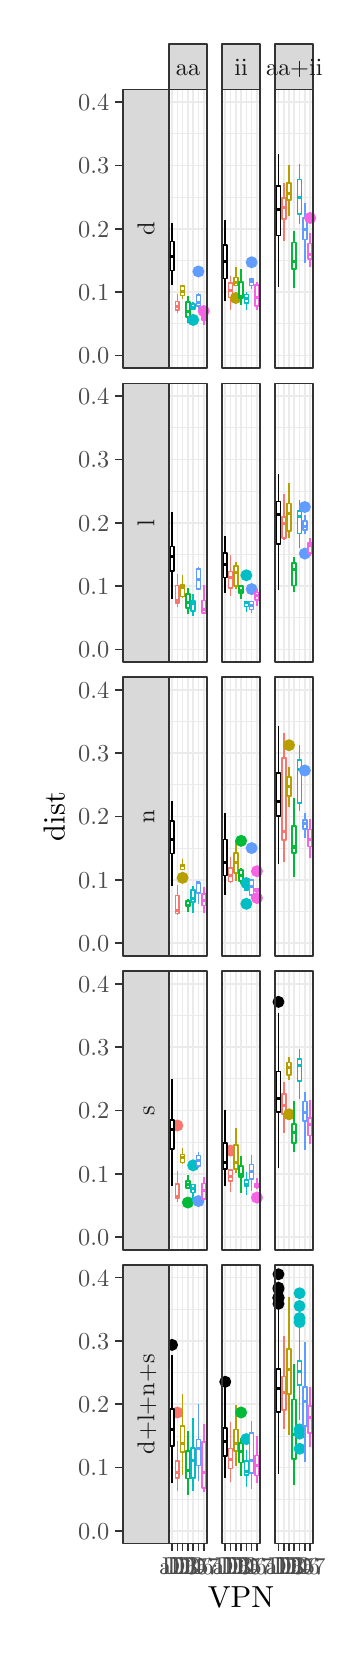
\begin{tikzpicture}[x=1pt,y=1pt]
\definecolor{fillColor}{RGB}{255,255,255}
\begin{scope}
\definecolor{drawColor}{RGB}{255,255,255}
\definecolor{fillColor}{RGB}{255,255,255}

\path[draw=drawColor,line width= 0.6pt,line join=round,line cap=round,fill=fillColor] (  0.00,  0.00) rectangle (108.41,578.16);
\end{scope}
\begin{scope}
\definecolor{fillColor}{RGB}{255,255,255}

\path[fill=fillColor] ( 50.73,455.41) rectangle ( 64.45,556.09);
\definecolor{drawColor}{gray}{0.92}

\path[draw=drawColor,line width= 0.3pt,line join=round] ( 50.73,471.43) --
	( 64.45,471.43);

\path[draw=drawColor,line width= 0.3pt,line join=round] ( 50.73,494.31) --
	( 64.45,494.31);

\path[draw=drawColor,line width= 0.3pt,line join=round] ( 50.73,517.19) --
	( 64.45,517.19);

\path[draw=drawColor,line width= 0.3pt,line join=round] ( 50.73,540.07) --
	( 64.45,540.07);

\path[draw=drawColor,line width= 0.6pt,line join=round] ( 50.73,459.98) --
	( 64.45,459.98);

\path[draw=drawColor,line width= 0.6pt,line join=round] ( 50.73,482.87) --
	( 64.45,482.87);

\path[draw=drawColor,line width= 0.6pt,line join=round] ( 50.73,505.75) --
	( 64.45,505.75);

\path[draw=drawColor,line width= 0.6pt,line join=round] ( 50.73,528.63) --
	( 64.45,528.63);

\path[draw=drawColor,line width= 0.6pt,line join=round] ( 50.73,551.51) --
	( 64.45,551.51);

\path[draw=drawColor,line width= 0.6pt,line join=round] ( 51.87,455.41) --
	( 51.87,556.09);

\path[draw=drawColor,line width= 0.6pt,line join=round] ( 53.78,455.41) --
	( 53.78,556.09);

\path[draw=drawColor,line width= 0.6pt,line join=round] ( 55.68,455.41) --
	( 55.68,556.09);

\path[draw=drawColor,line width= 0.6pt,line join=round] ( 57.59,455.41) --
	( 57.59,556.09);

\path[draw=drawColor,line width= 0.6pt,line join=round] ( 59.50,455.41) --
	( 59.50,556.09);

\path[draw=drawColor,line width= 0.6pt,line join=round] ( 61.40,455.41) --
	( 61.40,556.09);

\path[draw=drawColor,line width= 0.6pt,line join=round] ( 63.31,455.41) --
	( 63.31,556.09);
\definecolor{drawColor}{RGB}{248,118,109}

\path[draw=drawColor,line width= 0.6pt,line join=round] ( 53.78,479.45) -- ( 53.78,482.29);

\path[draw=drawColor,line width= 0.6pt,line join=round] ( 53.78,476.41) -- ( 53.78,475.43);

\path[draw=drawColor,line width= 0.6pt,line join=round,line cap=round,fill=fillColor] ( 53.06,479.45) --
	( 53.06,476.41) --
	( 54.49,476.41) --
	( 54.49,479.45) --
	( 53.06,479.45) --
	cycle;

\path[draw=drawColor,line width= 1.1pt,line join=round] ( 53.06,477.87) -- ( 54.49,477.87);
\definecolor{drawColor}{RGB}{183,159,0}

\path[draw=drawColor,line width= 0.6pt,line join=round] ( 55.68,485.11) -- ( 55.68,485.51);

\path[draw=drawColor,line width= 0.6pt,line join=round] ( 55.68,481.64) -- ( 55.68,480.31);

\path[draw=drawColor,line width= 0.6pt,line join=round,line cap=round,fill=fillColor] ( 54.97,485.11) --
	( 54.97,481.64) --
	( 56.40,481.64) --
	( 56.40,485.11) --
	( 54.97,485.11) --
	cycle;

\path[draw=drawColor,line width= 1.1pt,line join=round] ( 54.97,483.13) -- ( 56.40,483.13);
\definecolor{drawColor}{RGB}{0,186,56}

\path[draw=drawColor,line width= 0.6pt,line join=round] ( 57.59,479.31) -- ( 57.59,481.55);

\path[draw=drawColor,line width= 0.6pt,line join=round] ( 57.59,473.97) -- ( 57.59,471.90);

\path[draw=drawColor,line width= 0.6pt,line join=round,line cap=round,fill=fillColor] ( 56.88,479.31) --
	( 56.88,473.97) --
	( 58.31,473.97) --
	( 58.31,479.31) --
	( 56.88,479.31) --
	cycle;

\path[draw=drawColor,line width= 1.1pt,line join=round] ( 56.88,475.95) -- ( 58.31,475.95);
\definecolor{drawColor}{RGB}{0,191,196}
\definecolor{fillColor}{RGB}{0,191,196}

\path[draw=drawColor,line width= 0.4pt,line join=round,line cap=round,fill=fillColor] ( 59.50,472.85) circle (  1.96);

\path[draw=drawColor,line width= 0.6pt,line join=round] ( 59.50,478.62) -- ( 59.50,479.46);

\path[draw=drawColor,line width= 0.6pt,line join=round] ( 59.50,476.79) -- ( 59.50,476.76);
\definecolor{fillColor}{RGB}{255,255,255}

\path[draw=drawColor,line width= 0.6pt,line join=round,line cap=round,fill=fillColor] ( 58.78,478.62) --
	( 58.78,476.79) --
	( 60.21,476.79) --
	( 60.21,478.62) --
	( 58.78,478.62) --
	cycle;

\path[draw=drawColor,line width= 1.1pt,line join=round] ( 58.78,477.22) -- ( 60.21,477.22);
\definecolor{drawColor}{RGB}{97,156,255}
\definecolor{fillColor}{RGB}{97,156,255}

\path[draw=drawColor,line width= 0.4pt,line join=round,line cap=round,fill=fillColor] ( 61.40,490.36) circle (  1.96);

\path[draw=drawColor,line width= 0.6pt,line join=round] ( 61.40,481.95) -- ( 61.40,482.64);

\path[draw=drawColor,line width= 0.6pt,line join=round] ( 61.40,477.77) -- ( 61.40,475.77);
\definecolor{fillColor}{RGB}{255,255,255}

\path[draw=drawColor,line width= 0.6pt,line join=round,line cap=round,fill=fillColor] ( 60.69,481.95) --
	( 60.69,477.77) --
	( 62.12,477.77) --
	( 62.12,481.95) --
	( 60.69,481.95) --
	cycle;

\path[draw=drawColor,line width= 1.1pt,line join=round] ( 60.69,479.05) -- ( 62.12,479.05);
\definecolor{drawColor}{RGB}{245,100,227}
\definecolor{fillColor}{RGB}{245,100,227}

\path[draw=drawColor,line width= 0.4pt,line join=round,line cap=round,fill=fillColor] ( 63.31,476.07) circle (  1.96);

\path[draw=drawColor,line width= 0.6pt,line join=round] ( 63.31,474.03) -- ( 63.31,474.13);

\path[draw=drawColor,line width= 0.6pt,line join=round] ( 63.31,472.83) -- ( 63.31,471.18);
\definecolor{fillColor}{RGB}{255,255,255}

\path[draw=drawColor,line width= 0.6pt,line join=round,line cap=round,fill=fillColor] ( 62.59,474.03) --
	( 62.59,472.83) --
	( 64.02,472.83) --
	( 64.02,474.03) --
	( 62.59,474.03) --
	cycle;

\path[draw=drawColor,line width= 1.1pt,line join=round] ( 62.59,473.58) -- ( 64.02,473.58);
\definecolor{drawColor}{RGB}{0,0,0}

\path[draw=drawColor,line width= 0.6pt,line join=round] ( 51.87,501.17) -- ( 51.87,507.77);

\path[draw=drawColor,line width= 0.6pt,line join=round] ( 51.87,490.70) -- ( 51.87,485.37);

\path[draw=drawColor,line width= 0.6pt,line join=round,line cap=round,fill=fillColor] ( 51.16,501.17) --
	( 51.16,490.70) --
	( 52.59,490.70) --
	( 52.59,501.17) --
	( 51.16,501.17) --
	cycle;

\path[draw=drawColor,line width= 1.1pt,line join=round] ( 51.16,495.63) -- ( 52.59,495.63);
\definecolor{drawColor}{gray}{0.20}

\path[draw=drawColor,line width= 0.6pt,line join=round,line cap=round] ( 50.73,455.41) rectangle ( 64.45,556.09);
\end{scope}
\begin{scope}
\definecolor{fillColor}{RGB}{255,255,255}

\path[fill=fillColor] ( 50.73,349.23) rectangle ( 64.45,449.91);
\definecolor{drawColor}{gray}{0.92}

\path[draw=drawColor,line width= 0.3pt,line join=round] ( 50.73,365.24) --
	( 64.45,365.24);

\path[draw=drawColor,line width= 0.3pt,line join=round] ( 50.73,388.13) --
	( 64.45,388.13);

\path[draw=drawColor,line width= 0.3pt,line join=round] ( 50.73,411.01) --
	( 64.45,411.01);

\path[draw=drawColor,line width= 0.3pt,line join=round] ( 50.73,433.89) --
	( 64.45,433.89);

\path[draw=drawColor,line width= 0.6pt,line join=round] ( 50.73,353.80) --
	( 64.45,353.80);

\path[draw=drawColor,line width= 0.6pt,line join=round] ( 50.73,376.69) --
	( 64.45,376.69);

\path[draw=drawColor,line width= 0.6pt,line join=round] ( 50.73,399.57) --
	( 64.45,399.57);

\path[draw=drawColor,line width= 0.6pt,line join=round] ( 50.73,422.45) --
	( 64.45,422.45);

\path[draw=drawColor,line width= 0.6pt,line join=round] ( 50.73,445.33) --
	( 64.45,445.33);

\path[draw=drawColor,line width= 0.6pt,line join=round] ( 51.87,349.23) --
	( 51.87,449.91);

\path[draw=drawColor,line width= 0.6pt,line join=round] ( 53.78,349.23) --
	( 53.78,449.91);

\path[draw=drawColor,line width= 0.6pt,line join=round] ( 55.68,349.23) --
	( 55.68,449.91);

\path[draw=drawColor,line width= 0.6pt,line join=round] ( 57.59,349.23) --
	( 57.59,449.91);

\path[draw=drawColor,line width= 0.6pt,line join=round] ( 59.50,349.23) --
	( 59.50,449.91);

\path[draw=drawColor,line width= 0.6pt,line join=round] ( 61.40,349.23) --
	( 61.40,449.91);

\path[draw=drawColor,line width= 0.6pt,line join=round] ( 63.31,349.23) --
	( 63.31,449.91);
\definecolor{drawColor}{RGB}{248,118,109}

\path[draw=drawColor,line width= 0.6pt,line join=round] ( 53.78,376.88) -- ( 53.78,380.94);

\path[draw=drawColor,line width= 0.6pt,line join=round] ( 53.78,370.51) -- ( 53.78,369.09);

\path[draw=drawColor,line width= 0.6pt,line join=round,line cap=round,fill=fillColor] ( 53.06,376.88) --
	( 53.06,370.51) --
	( 54.49,370.51) --
	( 54.49,376.88) --
	( 53.06,376.88) --
	cycle;

\path[draw=drawColor,line width= 1.1pt,line join=round] ( 53.06,371.61) -- ( 54.49,371.61);
\definecolor{drawColor}{RGB}{183,159,0}

\path[draw=drawColor,line width= 0.6pt,line join=round] ( 55.68,377.02) -- ( 55.68,380.56);

\path[draw=drawColor,line width= 0.6pt,line join=round] ( 55.68,372.90) -- ( 55.68,372.86);

\path[draw=drawColor,line width= 0.6pt,line join=round,line cap=round,fill=fillColor] ( 54.97,377.02) --
	( 54.97,372.90) --
	( 56.40,372.90) --
	( 56.40,377.02) --
	( 54.97,377.02) --
	cycle;

\path[draw=drawColor,line width= 1.1pt,line join=round] ( 54.97,376.10) -- ( 56.40,376.10);
\definecolor{drawColor}{RGB}{0,186,56}

\path[draw=drawColor,line width= 0.6pt,line join=round] ( 57.59,373.89) -- ( 57.59,376.13);

\path[draw=drawColor,line width= 0.6pt,line join=round] ( 57.59,368.83) -- ( 57.59,366.48);

\path[draw=drawColor,line width= 0.6pt,line join=round,line cap=round,fill=fillColor] ( 56.88,373.89) --
	( 56.88,368.83) --
	( 58.31,368.83) --
	( 58.31,373.89) --
	( 56.88,373.89) --
	cycle;

\path[draw=drawColor,line width= 1.1pt,line join=round] ( 56.88,370.85) -- ( 58.31,370.85);
\definecolor{drawColor}{RGB}{0,191,196}

\path[draw=drawColor,line width= 0.6pt,line join=round] ( 59.50,371.23) -- ( 59.50,373.66);

\path[draw=drawColor,line width= 0.6pt,line join=round] ( 59.50,367.66) -- ( 59.50,366.02);

\path[draw=drawColor,line width= 0.6pt,line join=round,line cap=round,fill=fillColor] ( 58.78,371.23) --
	( 58.78,367.66) --
	( 60.21,367.66) --
	( 60.21,371.23) --
	( 58.78,371.23) --
	cycle;

\path[draw=drawColor,line width= 1.1pt,line join=round] ( 58.78,370.36) -- ( 60.21,370.36);
\definecolor{drawColor}{RGB}{97,156,255}

\path[draw=drawColor,line width= 0.6pt,line join=round] ( 61.40,382.95) -- ( 61.40,383.63);

\path[draw=drawColor,line width= 0.6pt,line join=round] ( 61.40,375.66) -- ( 61.40,375.50);

\path[draw=drawColor,line width= 0.6pt,line join=round,line cap=round,fill=fillColor] ( 60.69,382.95) --
	( 60.69,375.66) --
	( 62.12,375.66) --
	( 62.12,382.95) --
	( 60.69,382.95) --
	cycle;

\path[draw=drawColor,line width= 1.1pt,line join=round] ( 60.69,379.12) -- ( 62.12,379.12);
\definecolor{drawColor}{RGB}{245,100,227}

\path[draw=drawColor,line width= 0.6pt,line join=round] ( 63.31,371.41) -- ( 63.31,377.12);

\path[draw=drawColor,line width= 0.6pt,line join=round] ( 63.31,367.05) -- ( 63.31,366.81);

\path[draw=drawColor,line width= 0.6pt,line join=round,line cap=round,fill=fillColor] ( 62.59,371.41) --
	( 62.59,367.05) --
	( 64.02,367.05) --
	( 64.02,371.41) --
	( 62.59,371.41) --
	cycle;

\path[draw=drawColor,line width= 1.1pt,line join=round] ( 62.59,368.23) -- ( 64.02,368.23);
\definecolor{drawColor}{RGB}{0,0,0}

\path[draw=drawColor,line width= 0.6pt,line join=round] ( 51.87,391.03) -- ( 51.87,403.31);

\path[draw=drawColor,line width= 0.6pt,line join=round] ( 51.87,382.10) -- ( 51.87,371.89);

\path[draw=drawColor,line width= 0.6pt,line join=round,line cap=round,fill=fillColor] ( 51.16,391.03) --
	( 51.16,382.10) --
	( 52.59,382.10) --
	( 52.59,391.03) --
	( 51.16,391.03) --
	cycle;

\path[draw=drawColor,line width= 1.1pt,line join=round] ( 51.16,387.29) -- ( 52.59,387.29);
\definecolor{drawColor}{gray}{0.20}

\path[draw=drawColor,line width= 0.6pt,line join=round,line cap=round] ( 50.73,349.23) rectangle ( 64.45,449.91);
\end{scope}
\begin{scope}
\definecolor{fillColor}{RGB}{255,255,255}

\path[fill=fillColor] ( 50.73,243.05) rectangle ( 64.45,343.73);
\definecolor{drawColor}{gray}{0.92}

\path[draw=drawColor,line width= 0.3pt,line join=round] ( 50.73,259.06) --
	( 64.45,259.06);

\path[draw=drawColor,line width= 0.3pt,line join=round] ( 50.73,281.95) --
	( 64.45,281.95);

\path[draw=drawColor,line width= 0.3pt,line join=round] ( 50.73,304.83) --
	( 64.45,304.83);

\path[draw=drawColor,line width= 0.3pt,line join=round] ( 50.73,327.71) --
	( 64.45,327.71);

\path[draw=drawColor,line width= 0.6pt,line join=round] ( 50.73,247.62) --
	( 64.45,247.62);

\path[draw=drawColor,line width= 0.6pt,line join=round] ( 50.73,270.51) --
	( 64.45,270.51);

\path[draw=drawColor,line width= 0.6pt,line join=round] ( 50.73,293.39) --
	( 64.45,293.39);

\path[draw=drawColor,line width= 0.6pt,line join=round] ( 50.73,316.27) --
	( 64.45,316.27);

\path[draw=drawColor,line width= 0.6pt,line join=round] ( 50.73,339.15) --
	( 64.45,339.15);

\path[draw=drawColor,line width= 0.6pt,line join=round] ( 51.87,243.05) --
	( 51.87,343.73);

\path[draw=drawColor,line width= 0.6pt,line join=round] ( 53.78,243.05) --
	( 53.78,343.73);

\path[draw=drawColor,line width= 0.6pt,line join=round] ( 55.68,243.05) --
	( 55.68,343.73);

\path[draw=drawColor,line width= 0.6pt,line join=round] ( 57.59,243.05) --
	( 57.59,343.73);

\path[draw=drawColor,line width= 0.6pt,line join=round] ( 59.50,243.05) --
	( 59.50,343.73);

\path[draw=drawColor,line width= 0.6pt,line join=round] ( 61.40,243.05) --
	( 61.40,343.73);

\path[draw=drawColor,line width= 0.6pt,line join=round] ( 63.31,243.05) --
	( 63.31,343.73);
\definecolor{drawColor}{RGB}{248,118,109}

\path[draw=drawColor,line width= 0.6pt,line join=round] ( 53.78,264.89) -- ( 53.78,268.70);

\path[draw=drawColor,line width= 0.6pt,line join=round] ( 53.78,258.31) -- ( 53.78,257.90);

\path[draw=drawColor,line width= 0.6pt,line join=round,line cap=round,fill=fillColor] ( 53.06,264.89) --
	( 53.06,258.31) --
	( 54.49,258.31) --
	( 54.49,264.89) --
	( 53.06,264.89) --
	cycle;

\path[draw=drawColor,line width= 1.1pt,line join=round] ( 53.06,259.46) -- ( 54.49,259.46);
\definecolor{drawColor}{RGB}{183,159,0}
\definecolor{fillColor}{RGB}{183,159,0}

\path[draw=drawColor,line width= 0.4pt,line join=round,line cap=round,fill=fillColor] ( 55.68,271.25) circle (  1.96);

\path[draw=drawColor,line width= 0.6pt,line join=round] ( 55.68,275.83) -- ( 55.68,277.99);

\path[draw=drawColor,line width= 0.6pt,line join=round] ( 55.68,274.24) -- ( 55.68,274.24);
\definecolor{fillColor}{RGB}{255,255,255}

\path[draw=drawColor,line width= 0.6pt,line join=round,line cap=round,fill=fillColor] ( 54.97,275.83) --
	( 54.97,274.24) --
	( 56.40,274.24) --
	( 56.40,275.83) --
	( 54.97,275.83) --
	cycle;

\path[draw=drawColor,line width= 1.1pt,line join=round] ( 54.97,275.70) -- ( 56.40,275.70);
\definecolor{drawColor}{RGB}{0,186,56}

\path[draw=drawColor,line width= 0.6pt,line join=round] ( 57.59,262.85) -- ( 57.59,263.73);

\path[draw=drawColor,line width= 0.6pt,line join=round] ( 57.59,261.03) -- ( 57.59,258.96);

\path[draw=drawColor,line width= 0.6pt,line join=round,line cap=round,fill=fillColor] ( 56.88,262.85) --
	( 56.88,261.03) --
	( 58.31,261.03) --
	( 58.31,262.85) --
	( 56.88,262.85) --
	cycle;

\path[draw=drawColor,line width= 1.1pt,line join=round] ( 56.88,261.28) -- ( 58.31,261.28);
\definecolor{drawColor}{RGB}{0,191,196}

\path[draw=drawColor,line width= 0.6pt,line join=round] ( 59.50,266.81) -- ( 59.50,268.18);

\path[draw=drawColor,line width= 0.6pt,line join=round] ( 59.50,262.53) -- ( 59.50,258.41);

\path[draw=drawColor,line width= 0.6pt,line join=round,line cap=round,fill=fillColor] ( 58.78,266.81) --
	( 58.78,262.53) --
	( 60.21,262.53) --
	( 60.21,266.81) --
	( 58.78,266.81) --
	cycle;

\path[draw=drawColor,line width= 1.1pt,line join=round] ( 58.78,263.68) -- ( 60.21,263.68);
\definecolor{drawColor}{RGB}{97,156,255}

\path[draw=drawColor,line width= 0.6pt,line join=round] ( 61.40,269.57) -- ( 61.40,270.14);

\path[draw=drawColor,line width= 0.6pt,line join=round] ( 61.40,265.72) -- ( 61.40,261.89);

\path[draw=drawColor,line width= 0.6pt,line join=round,line cap=round,fill=fillColor] ( 60.69,269.57) --
	( 60.69,265.72) --
	( 62.12,265.72) --
	( 62.12,269.57) --
	( 60.69,269.57) --
	cycle;

\path[draw=drawColor,line width= 1.1pt,line join=round] ( 60.69,269.43) -- ( 62.12,269.43);
\definecolor{drawColor}{RGB}{245,100,227}

\path[draw=drawColor,line width= 0.6pt,line join=round] ( 63.31,265.30) -- ( 63.31,268.10);

\path[draw=drawColor,line width= 0.6pt,line join=round] ( 63.31,261.26) -- ( 63.31,258.45);

\path[draw=drawColor,line width= 0.6pt,line join=round,line cap=round,fill=fillColor] ( 62.59,265.30) --
	( 62.59,261.26) --
	( 64.02,261.26) --
	( 64.02,265.30) --
	( 62.59,265.30) --
	cycle;

\path[draw=drawColor,line width= 1.1pt,line join=round] ( 62.59,263.09) -- ( 64.02,263.09);
\definecolor{drawColor}{RGB}{0,0,0}

\path[draw=drawColor,line width= 0.6pt,line join=round] ( 51.87,291.78) -- ( 51.87,298.88);

\path[draw=drawColor,line width= 0.6pt,line join=round] ( 51.87,280.04) -- ( 51.87,268.39);

\path[draw=drawColor,line width= 0.6pt,line join=round,line cap=round,fill=fillColor] ( 51.16,291.78) --
	( 51.16,280.04) --
	( 52.59,280.04) --
	( 52.59,291.78) --
	( 51.16,291.78) --
	cycle;

\path[draw=drawColor,line width= 1.1pt,line join=round] ( 51.16,285.26) -- ( 52.59,285.26);
\definecolor{drawColor}{gray}{0.20}

\path[draw=drawColor,line width= 0.6pt,line join=round,line cap=round] ( 50.73,243.05) rectangle ( 64.45,343.73);
\end{scope}
\begin{scope}
\definecolor{fillColor}{RGB}{255,255,255}

\path[fill=fillColor] ( 50.73,136.87) rectangle ( 64.45,237.55);
\definecolor{drawColor}{gray}{0.92}

\path[draw=drawColor,line width= 0.3pt,line join=round] ( 50.73,152.88) --
	( 64.45,152.88);

\path[draw=drawColor,line width= 0.3pt,line join=round] ( 50.73,175.77) --
	( 64.45,175.77);

\path[draw=drawColor,line width= 0.3pt,line join=round] ( 50.73,198.65) --
	( 64.45,198.65);

\path[draw=drawColor,line width= 0.3pt,line join=round] ( 50.73,221.53) --
	( 64.45,221.53);

\path[draw=drawColor,line width= 0.6pt,line join=round] ( 50.73,141.44) --
	( 64.45,141.44);

\path[draw=drawColor,line width= 0.6pt,line join=round] ( 50.73,164.32) --
	( 64.45,164.32);

\path[draw=drawColor,line width= 0.6pt,line join=round] ( 50.73,187.21) --
	( 64.45,187.21);

\path[draw=drawColor,line width= 0.6pt,line join=round] ( 50.73,210.09) --
	( 64.45,210.09);

\path[draw=drawColor,line width= 0.6pt,line join=round] ( 50.73,232.97) --
	( 64.45,232.97);

\path[draw=drawColor,line width= 0.6pt,line join=round] ( 51.87,136.87) --
	( 51.87,237.55);

\path[draw=drawColor,line width= 0.6pt,line join=round] ( 53.78,136.87) --
	( 53.78,237.55);

\path[draw=drawColor,line width= 0.6pt,line join=round] ( 55.68,136.87) --
	( 55.68,237.55);

\path[draw=drawColor,line width= 0.6pt,line join=round] ( 57.59,136.87) --
	( 57.59,237.55);

\path[draw=drawColor,line width= 0.6pt,line join=round] ( 59.50,136.87) --
	( 59.50,237.55);

\path[draw=drawColor,line width= 0.6pt,line join=round] ( 61.40,136.87) --
	( 61.40,237.55);

\path[draw=drawColor,line width= 0.6pt,line join=round] ( 63.31,136.87) --
	( 63.31,237.55);
\definecolor{drawColor}{RGB}{248,118,109}
\definecolor{fillColor}{RGB}{248,118,109}

\path[draw=drawColor,line width= 0.4pt,line join=round,line cap=round,fill=fillColor] ( 53.78,181.75) circle (  1.96);

\path[draw=drawColor,line width= 0.6pt,line join=round] ( 53.78,160.50) -- ( 53.78,165.22);

\path[draw=drawColor,line width= 0.6pt,line join=round] ( 53.78,155.58) -- ( 53.78,153.98);
\definecolor{fillColor}{RGB}{255,255,255}

\path[draw=drawColor,line width= 0.6pt,line join=round,line cap=round,fill=fillColor] ( 53.06,160.50) --
	( 53.06,155.58) --
	( 54.49,155.58) --
	( 54.49,160.50) --
	( 53.06,160.50) --
	cycle;

\path[draw=drawColor,line width= 1.1pt,line join=round] ( 53.06,156.26) -- ( 54.49,156.26);
\definecolor{drawColor}{RGB}{183,159,0}

\path[draw=drawColor,line width= 0.6pt,line join=round] ( 55.68,171.28) -- ( 55.68,173.50);

\path[draw=drawColor,line width= 0.6pt,line join=round] ( 55.68,168.39) -- ( 55.68,167.88);

\path[draw=drawColor,line width= 0.6pt,line join=round,line cap=round,fill=fillColor] ( 54.97,171.28) --
	( 54.97,168.39) --
	( 56.40,168.39) --
	( 56.40,171.28) --
	( 54.97,171.28) --
	cycle;

\path[draw=drawColor,line width= 1.1pt,line join=round] ( 54.97,170.19) -- ( 56.40,170.19);
\definecolor{drawColor}{RGB}{0,186,56}
\definecolor{fillColor}{RGB}{0,186,56}

\path[draw=drawColor,line width= 0.4pt,line join=round,line cap=round,fill=fillColor] ( 57.59,153.92) circle (  1.96);

\path[draw=drawColor,line width= 0.6pt,line join=round] ( 57.59,161.73) -- ( 57.59,164.00);

\path[draw=drawColor,line width= 0.6pt,line join=round] ( 57.59,159.29) -- ( 57.59,158.94);
\definecolor{fillColor}{RGB}{255,255,255}

\path[draw=drawColor,line width= 0.6pt,line join=round,line cap=round,fill=fillColor] ( 56.88,161.73) --
	( 56.88,159.29) --
	( 58.31,159.29) --
	( 58.31,161.73) --
	( 56.88,161.73) --
	cycle;

\path[draw=drawColor,line width= 1.1pt,line join=round] ( 56.88,160.39) -- ( 58.31,160.39);
\definecolor{drawColor}{RGB}{0,191,196}
\definecolor{fillColor}{RGB}{0,191,196}

\path[draw=drawColor,line width= 0.4pt,line join=round,line cap=round,fill=fillColor] ( 59.50,167.36) circle (  1.96);

\path[draw=drawColor,line width= 0.6pt,line join=round] ( 59.50,160.45) -- ( 59.50,160.79);

\path[draw=drawColor,line width= 0.6pt,line join=round] ( 59.50,157.52) -- ( 59.50,154.57);
\definecolor{fillColor}{RGB}{255,255,255}

\path[draw=drawColor,line width= 0.6pt,line join=round,line cap=round,fill=fillColor] ( 58.78,160.45) --
	( 58.78,157.52) --
	( 60.21,157.52) --
	( 60.21,160.45) --
	( 58.78,160.45) --
	cycle;

\path[draw=drawColor,line width= 1.1pt,line join=round] ( 58.78,159.10) -- ( 60.21,159.10);
\definecolor{drawColor}{RGB}{97,156,255}
\definecolor{fillColor}{RGB}{97,156,255}

\path[draw=drawColor,line width= 0.4pt,line join=round,line cap=round,fill=fillColor] ( 61.40,154.45) circle (  1.96);

\path[draw=drawColor,line width= 0.6pt,line join=round] ( 61.40,170.95) -- ( 61.40,172.34);

\path[draw=drawColor,line width= 0.6pt,line join=round] ( 61.40,167.09) -- ( 61.40,166.53);
\definecolor{fillColor}{RGB}{255,255,255}

\path[draw=drawColor,line width= 0.6pt,line join=round,line cap=round,fill=fillColor] ( 60.69,170.95) --
	( 60.69,167.09) --
	( 62.12,167.09) --
	( 62.12,170.95) --
	( 60.69,170.95) --
	cycle;

\path[draw=drawColor,line width= 1.1pt,line join=round] ( 60.69,169.07) -- ( 62.12,169.07);
\definecolor{drawColor}{RGB}{245,100,227}

\path[draw=drawColor,line width= 0.6pt,line join=round] ( 63.31,160.81) -- ( 63.31,163.10);

\path[draw=drawColor,line width= 0.6pt,line join=round] ( 63.31,155.17) -- ( 63.31,154.75);

\path[draw=drawColor,line width= 0.6pt,line join=round,line cap=round,fill=fillColor] ( 62.59,160.81) --
	( 62.59,155.17) --
	( 64.02,155.17) --
	( 64.02,160.81) --
	( 62.59,160.81) --
	cycle;

\path[draw=drawColor,line width= 1.1pt,line join=round] ( 62.59,158.15) -- ( 64.02,158.15);
\definecolor{drawColor}{RGB}{0,0,0}

\path[draw=drawColor,line width= 0.6pt,line join=round] ( 51.87,183.66) -- ( 51.87,198.69);

\path[draw=drawColor,line width= 0.6pt,line join=round] ( 51.87,173.36) -- ( 51.87,159.76);

\path[draw=drawColor,line width= 0.6pt,line join=round,line cap=round,fill=fillColor] ( 51.16,183.66) --
	( 51.16,173.36) --
	( 52.59,173.36) --
	( 52.59,183.66) --
	( 51.16,183.66) --
	cycle;

\path[draw=drawColor,line width= 1.1pt,line join=round] ( 51.16,180.39) -- ( 52.59,180.39);
\definecolor{drawColor}{gray}{0.20}

\path[draw=drawColor,line width= 0.6pt,line join=round,line cap=round] ( 50.73,136.87) rectangle ( 64.45,237.55);
\end{scope}
\begin{scope}
\definecolor{fillColor}{RGB}{255,255,255}

\path[fill=fillColor] ( 50.73, 30.69) rectangle ( 64.45,131.37);
\definecolor{drawColor}{gray}{0.92}

\path[draw=drawColor,line width= 0.3pt,line join=round] ( 50.73, 46.70) --
	( 64.45, 46.70);

\path[draw=drawColor,line width= 0.3pt,line join=round] ( 50.73, 69.59) --
	( 64.45, 69.59);

\path[draw=drawColor,line width= 0.3pt,line join=round] ( 50.73, 92.47) --
	( 64.45, 92.47);

\path[draw=drawColor,line width= 0.3pt,line join=round] ( 50.73,115.35) --
	( 64.45,115.35);

\path[draw=drawColor,line width= 0.6pt,line join=round] ( 50.73, 35.26) --
	( 64.45, 35.26);

\path[draw=drawColor,line width= 0.6pt,line join=round] ( 50.73, 58.14) --
	( 64.45, 58.14);

\path[draw=drawColor,line width= 0.6pt,line join=round] ( 50.73, 81.03) --
	( 64.45, 81.03);

\path[draw=drawColor,line width= 0.6pt,line join=round] ( 50.73,103.91) --
	( 64.45,103.91);

\path[draw=drawColor,line width= 0.6pt,line join=round] ( 50.73,126.79) --
	( 64.45,126.79);

\path[draw=drawColor,line width= 0.6pt,line join=round] ( 51.87, 30.69) --
	( 51.87,131.37);

\path[draw=drawColor,line width= 0.6pt,line join=round] ( 53.78, 30.69) --
	( 53.78,131.37);

\path[draw=drawColor,line width= 0.6pt,line join=round] ( 55.68, 30.69) --
	( 55.68,131.37);

\path[draw=drawColor,line width= 0.6pt,line join=round] ( 57.59, 30.69) --
	( 57.59,131.37);

\path[draw=drawColor,line width= 0.6pt,line join=round] ( 59.50, 30.69) --
	( 59.50,131.37);

\path[draw=drawColor,line width= 0.6pt,line join=round] ( 61.40, 30.69) --
	( 61.40,131.37);

\path[draw=drawColor,line width= 0.6pt,line join=round] ( 63.31, 30.69) --
	( 63.31,131.37);
\definecolor{drawColor}{RGB}{248,118,109}
\definecolor{fillColor}{RGB}{248,118,109}

\path[draw=drawColor,line width= 0.4pt,line join=round,line cap=round,fill=fillColor] ( 53.78, 78.04) circle (  1.96);

\path[draw=drawColor,line width= 0.6pt,line join=round] ( 53.78, 60.51) -- ( 53.78, 67.59);

\path[draw=drawColor,line width= 0.6pt,line join=round] ( 53.78, 54.48) -- ( 53.78, 49.58);
\definecolor{fillColor}{RGB}{255,255,255}

\path[draw=drawColor,line width= 0.6pt,line join=round,line cap=round,fill=fillColor] ( 53.06, 60.51) --
	( 53.06, 54.48) --
	( 54.49, 54.48) --
	( 54.49, 60.51) --
	( 53.06, 60.51) --
	cycle;

\path[draw=drawColor,line width= 1.1pt,line join=round] ( 53.06, 56.20) -- ( 54.49, 56.20);
\definecolor{drawColor}{RGB}{183,159,0}

\path[draw=drawColor,line width= 0.6pt,line join=round] ( 55.68, 73.10) -- ( 55.68, 84.61);

\path[draw=drawColor,line width= 0.6pt,line join=round] ( 55.68, 63.68) -- ( 55.68, 55.43);

\path[draw=drawColor,line width= 0.6pt,line join=round,line cap=round,fill=fillColor] ( 54.97, 73.10) --
	( 54.97, 63.68) --
	( 56.40, 63.68) --
	( 56.40, 73.10) --
	( 54.97, 73.10) --
	cycle;

\path[draw=drawColor,line width= 1.1pt,line join=round] ( 54.97, 66.93) -- ( 56.40, 66.93);
\definecolor{drawColor}{RGB}{0,186,56}

\path[draw=drawColor,line width= 0.6pt,line join=round] ( 57.59, 64.22) -- ( 57.59, 71.42);

\path[draw=drawColor,line width= 0.6pt,line join=round] ( 57.59, 54.21) -- ( 57.59, 48.29);

\path[draw=drawColor,line width= 0.6pt,line join=round,line cap=round,fill=fillColor] ( 56.88, 64.22) --
	( 56.88, 54.21) --
	( 58.31, 54.21) --
	( 58.31, 64.22) --
	( 56.88, 64.22) --
	cycle;

\path[draw=drawColor,line width= 1.1pt,line join=round] ( 56.88, 57.17) -- ( 58.31, 57.17);
\definecolor{drawColor}{RGB}{0,191,196}

\path[draw=drawColor,line width= 0.6pt,line join=round] ( 59.50, 65.29) -- ( 59.50, 75.97);

\path[draw=drawColor,line width= 0.6pt,line join=round] ( 59.50, 54.46) -- ( 59.50, 49.67);

\path[draw=drawColor,line width= 0.6pt,line join=round,line cap=round,fill=fillColor] ( 58.78, 65.29) --
	( 58.78, 54.46) --
	( 60.21, 54.46) --
	( 60.21, 65.29) --
	( 58.78, 65.29) --
	cycle;

\path[draw=drawColor,line width= 1.1pt,line join=round] ( 58.78, 60.57) -- ( 60.21, 60.57);
\definecolor{drawColor}{RGB}{97,156,255}

\path[draw=drawColor,line width= 0.6pt,line join=round] ( 61.40, 68.29) -- ( 61.40, 81.28);

\path[draw=drawColor,line width= 0.6pt,line join=round] ( 61.40, 58.93) -- ( 61.40, 53.17);

\path[draw=drawColor,line width= 0.6pt,line join=round,line cap=round,fill=fillColor] ( 60.69, 68.29) --
	( 60.69, 58.93) --
	( 62.12, 58.93) --
	( 62.12, 68.29) --
	( 60.69, 68.29) --
	cycle;

\path[draw=drawColor,line width= 1.1pt,line join=round] ( 60.69, 64.88) -- ( 62.12, 64.88);
\definecolor{drawColor}{RGB}{245,100,227}

\path[draw=drawColor,line width= 0.6pt,line join=round] ( 63.31, 67.37) -- ( 63.31, 73.90);

\path[draw=drawColor,line width= 0.6pt,line join=round] ( 63.31, 50.68) -- ( 63.31, 49.47);

\path[draw=drawColor,line width= 0.6pt,line join=round,line cap=round,fill=fillColor] ( 62.59, 67.37) --
	( 62.59, 50.68) --
	( 64.02, 50.68) --
	( 64.02, 67.37) --
	( 62.59, 67.37) --
	cycle;

\path[draw=drawColor,line width= 1.1pt,line join=round] ( 62.59, 56.22) -- ( 64.02, 56.22);
\definecolor{drawColor}{RGB}{0,0,0}
\definecolor{fillColor}{RGB}{0,0,0}

\path[draw=drawColor,line width= 0.4pt,line join=round,line cap=round,fill=fillColor] ( 51.87,102.48) circle (  1.96);

\path[draw=drawColor,line width= 0.6pt,line join=round] ( 51.87, 79.29) -- ( 51.87, 98.88);

\path[draw=drawColor,line width= 0.6pt,line join=round] ( 51.87, 65.96) -- ( 51.87, 52.67);
\definecolor{fillColor}{RGB}{255,255,255}

\path[draw=drawColor,line width= 0.6pt,line join=round,line cap=round,fill=fillColor] ( 51.16, 79.29) --
	( 51.16, 65.96) --
	( 52.59, 65.96) --
	( 52.59, 79.29) --
	( 51.16, 79.29) --
	cycle;

\path[draw=drawColor,line width= 1.1pt,line join=round] ( 51.16, 71.78) -- ( 52.59, 71.78);
\definecolor{drawColor}{gray}{0.20}

\path[draw=drawColor,line width= 0.6pt,line join=round,line cap=round] ( 50.73, 30.69) rectangle ( 64.45,131.37);
\end{scope}
\begin{scope}
\definecolor{fillColor}{RGB}{255,255,255}

\path[fill=fillColor] ( 69.95,455.41) rectangle ( 83.68,556.09);
\definecolor{drawColor}{gray}{0.92}

\path[draw=drawColor,line width= 0.3pt,line join=round] ( 69.95,471.43) --
	( 83.68,471.43);

\path[draw=drawColor,line width= 0.3pt,line join=round] ( 69.95,494.31) --
	( 83.68,494.31);

\path[draw=drawColor,line width= 0.3pt,line join=round] ( 69.95,517.19) --
	( 83.68,517.19);

\path[draw=drawColor,line width= 0.3pt,line join=round] ( 69.95,540.07) --
	( 83.68,540.07);

\path[draw=drawColor,line width= 0.6pt,line join=round] ( 69.95,459.98) --
	( 83.68,459.98);

\path[draw=drawColor,line width= 0.6pt,line join=round] ( 69.95,482.87) --
	( 83.68,482.87);

\path[draw=drawColor,line width= 0.6pt,line join=round] ( 69.95,505.75) --
	( 83.68,505.75);

\path[draw=drawColor,line width= 0.6pt,line join=round] ( 69.95,528.63) --
	( 83.68,528.63);

\path[draw=drawColor,line width= 0.6pt,line join=round] ( 69.95,551.51) --
	( 83.68,551.51);

\path[draw=drawColor,line width= 0.6pt,line join=round] ( 71.10,455.41) --
	( 71.10,556.09);

\path[draw=drawColor,line width= 0.6pt,line join=round] ( 73.00,455.41) --
	( 73.00,556.09);

\path[draw=drawColor,line width= 0.6pt,line join=round] ( 74.91,455.41) --
	( 74.91,556.09);

\path[draw=drawColor,line width= 0.6pt,line join=round] ( 76.82,455.41) --
	( 76.82,556.09);

\path[draw=drawColor,line width= 0.6pt,line join=round] ( 78.72,455.41) --
	( 78.72,556.09);

\path[draw=drawColor,line width= 0.6pt,line join=round] ( 80.63,455.41) --
	( 80.63,556.09);

\path[draw=drawColor,line width= 0.6pt,line join=round] ( 82.54,455.41) --
	( 82.54,556.09);
\definecolor{drawColor}{RGB}{248,118,109}

\path[draw=drawColor,line width= 0.6pt,line join=round] ( 73.00,486.28) -- ( 73.00,488.63);

\path[draw=drawColor,line width= 0.6pt,line join=round] ( 73.00,481.01) -- ( 73.00,476.53);

\path[draw=drawColor,line width= 0.6pt,line join=round,line cap=round,fill=fillColor] ( 72.29,486.28) --
	( 72.29,481.01) --
	( 73.72,481.01) --
	( 73.72,486.28) --
	( 72.29,486.28) --
	cycle;

\path[draw=drawColor,line width= 1.1pt,line join=round] ( 72.29,483.50) -- ( 73.72,483.50);
\definecolor{drawColor}{RGB}{183,159,0}
\definecolor{fillColor}{RGB}{183,159,0}

\path[draw=drawColor,line width= 0.4pt,line join=round,line cap=round,fill=fillColor] ( 74.91,480.77) circle (  1.96);

\path[draw=drawColor,line width= 0.6pt,line join=round] ( 74.91,488.18) -- ( 74.91,492.08);

\path[draw=drawColor,line width= 0.6pt,line join=round] ( 74.91,485.29) -- ( 74.91,485.20);
\definecolor{fillColor}{RGB}{255,255,255}

\path[draw=drawColor,line width= 0.6pt,line join=round,line cap=round,fill=fillColor] ( 74.20,488.18) --
	( 74.20,485.29) --
	( 75.62,485.29) --
	( 75.62,488.18) --
	( 74.20,488.18) --
	cycle;

\path[draw=drawColor,line width= 1.1pt,line join=round] ( 74.20,486.27) -- ( 75.62,486.27);
\definecolor{drawColor}{RGB}{0,186,56}

\path[draw=drawColor,line width= 0.6pt,line join=round] ( 76.82,486.59) -- ( 76.82,491.17);

\path[draw=drawColor,line width= 0.6pt,line join=round] ( 76.82,480.88) -- ( 76.82,478.15);

\path[draw=drawColor,line width= 0.6pt,line join=round,line cap=round,fill=fillColor] ( 76.10,486.59) --
	( 76.10,480.88) --
	( 77.53,480.88) --
	( 77.53,486.59) --
	( 76.10,486.59) --
	cycle;

\path[draw=drawColor,line width= 1.1pt,line join=round] ( 76.10,481.32) -- ( 77.53,481.32);
\definecolor{drawColor}{RGB}{0,191,196}

\path[draw=drawColor,line width= 0.6pt,line join=round] ( 78.72,482.08) -- ( 78.72,483.02);

\path[draw=drawColor,line width= 0.6pt,line join=round] ( 78.72,478.98) -- ( 78.72,476.45);

\path[draw=drawColor,line width= 0.6pt,line join=round,line cap=round,fill=fillColor] ( 78.01,482.08) --
	( 78.01,478.98) --
	( 79.44,478.98) --
	( 79.44,482.08) --
	( 78.01,482.08) --
	cycle;

\path[draw=drawColor,line width= 1.1pt,line join=round] ( 78.01,480.68) -- ( 79.44,480.68);
\definecolor{drawColor}{RGB}{97,156,255}
\definecolor{fillColor}{RGB}{97,156,255}

\path[draw=drawColor,line width= 0.4pt,line join=round,line cap=round,fill=fillColor] ( 80.63,493.68) circle (  1.96);

\path[draw=drawColor,line width= 0.6pt,line join=round] ( 80.63,487.72) -- ( 80.63,488.07);

\path[draw=drawColor,line width= 0.6pt,line join=round] ( 80.63,485.23) -- ( 80.63,483.89);
\definecolor{fillColor}{RGB}{255,255,255}

\path[draw=drawColor,line width= 0.6pt,line join=round,line cap=round,fill=fillColor] ( 79.91,487.72) --
	( 79.91,485.23) --
	( 81.34,485.23) --
	( 81.34,487.72) --
	( 79.91,487.72) --
	cycle;

\path[draw=drawColor,line width= 1.1pt,line join=round] ( 79.91,486.63) -- ( 81.34,486.63);
\definecolor{drawColor}{RGB}{245,100,227}

\path[draw=drawColor,line width= 0.6pt,line join=round] ( 82.54,485.43) -- ( 82.54,486.42);

\path[draw=drawColor,line width= 0.6pt,line join=round] ( 82.54,477.84) -- ( 82.54,476.53);

\path[draw=drawColor,line width= 0.6pt,line join=round,line cap=round,fill=fillColor] ( 81.82,485.43) --
	( 81.82,477.84) --
	( 83.25,477.84) --
	( 83.25,485.43) --
	( 81.82,485.43) --
	cycle;

\path[draw=drawColor,line width= 1.1pt,line join=round] ( 81.82,480.90) -- ( 83.25,480.90);
\definecolor{drawColor}{RGB}{0,0,0}

\path[draw=drawColor,line width= 0.6pt,line join=round] ( 71.10,499.84) -- ( 71.10,508.95);

\path[draw=drawColor,line width= 0.6pt,line join=round] ( 71.10,487.76) -- ( 71.10,479.69);

\path[draw=drawColor,line width= 0.6pt,line join=round,line cap=round,fill=fillColor] ( 70.38,499.84) --
	( 70.38,487.76) --
	( 71.81,487.76) --
	( 71.81,499.84) --
	( 70.38,499.84) --
	cycle;

\path[draw=drawColor,line width= 1.1pt,line join=round] ( 70.38,493.87) -- ( 71.81,493.87);
\definecolor{drawColor}{gray}{0.20}

\path[draw=drawColor,line width= 0.6pt,line join=round,line cap=round] ( 69.95,455.41) rectangle ( 83.68,556.09);
\end{scope}
\begin{scope}
\definecolor{fillColor}{RGB}{255,255,255}

\path[fill=fillColor] ( 69.95,349.23) rectangle ( 83.68,449.91);
\definecolor{drawColor}{gray}{0.92}

\path[draw=drawColor,line width= 0.3pt,line join=round] ( 69.95,365.24) --
	( 83.68,365.24);

\path[draw=drawColor,line width= 0.3pt,line join=round] ( 69.95,388.13) --
	( 83.68,388.13);

\path[draw=drawColor,line width= 0.3pt,line join=round] ( 69.95,411.01) --
	( 83.68,411.01);

\path[draw=drawColor,line width= 0.3pt,line join=round] ( 69.95,433.89) --
	( 83.68,433.89);

\path[draw=drawColor,line width= 0.6pt,line join=round] ( 69.95,353.80) --
	( 83.68,353.80);

\path[draw=drawColor,line width= 0.6pt,line join=round] ( 69.95,376.69) --
	( 83.68,376.69);

\path[draw=drawColor,line width= 0.6pt,line join=round] ( 69.95,399.57) --
	( 83.68,399.57);

\path[draw=drawColor,line width= 0.6pt,line join=round] ( 69.95,422.45) --
	( 83.68,422.45);

\path[draw=drawColor,line width= 0.6pt,line join=round] ( 69.95,445.33) --
	( 83.68,445.33);

\path[draw=drawColor,line width= 0.6pt,line join=round] ( 71.10,349.23) --
	( 71.10,449.91);

\path[draw=drawColor,line width= 0.6pt,line join=round] ( 73.00,349.23) --
	( 73.00,449.91);

\path[draw=drawColor,line width= 0.6pt,line join=round] ( 74.91,349.23) --
	( 74.91,449.91);

\path[draw=drawColor,line width= 0.6pt,line join=round] ( 76.82,349.23) --
	( 76.82,449.91);

\path[draw=drawColor,line width= 0.6pt,line join=round] ( 78.72,349.23) --
	( 78.72,449.91);

\path[draw=drawColor,line width= 0.6pt,line join=round] ( 80.63,349.23) --
	( 80.63,449.91);

\path[draw=drawColor,line width= 0.6pt,line join=round] ( 82.54,349.23) --
	( 82.54,449.91);
\definecolor{drawColor}{RGB}{248,118,109}

\path[draw=drawColor,line width= 0.6pt,line join=round] ( 73.00,381.98) -- ( 73.00,387.94);

\path[draw=drawColor,line width= 0.6pt,line join=round] ( 73.00,376.02) -- ( 73.00,373.03);

\path[draw=drawColor,line width= 0.6pt,line join=round,line cap=round,fill=fillColor] ( 72.29,381.98) --
	( 72.29,376.02) --
	( 73.72,376.02) --
	( 73.72,381.98) --
	( 72.29,381.98) --
	cycle;

\path[draw=drawColor,line width= 1.1pt,line join=round] ( 72.29,379.78) -- ( 73.72,379.78);
\definecolor{drawColor}{RGB}{183,159,0}

\path[draw=drawColor,line width= 0.6pt,line join=round] ( 74.91,383.94) -- ( 74.91,385.51);

\path[draw=drawColor,line width= 0.6pt,line join=round] ( 74.91,376.80) -- ( 74.91,375.58);

\path[draw=drawColor,line width= 0.6pt,line join=round,line cap=round,fill=fillColor] ( 74.20,383.94) --
	( 74.20,376.80) --
	( 75.62,376.80) --
	( 75.62,383.94) --
	( 74.20,383.94) --
	cycle;

\path[draw=drawColor,line width= 1.1pt,line join=round] ( 74.20,381.75) -- ( 75.62,381.75);
\definecolor{drawColor}{RGB}{0,186,56}

\path[draw=drawColor,line width= 0.6pt,line join=round] ( 76.82,376.73) -- ( 76.82,377.16);

\path[draw=drawColor,line width= 0.6pt,line join=round] ( 76.82,374.20) -- ( 76.82,372.14);

\path[draw=drawColor,line width= 0.6pt,line join=round,line cap=round,fill=fillColor] ( 76.10,376.73) --
	( 76.10,374.20) --
	( 77.53,374.20) --
	( 77.53,376.73) --
	( 76.10,376.73) --
	cycle;

\path[draw=drawColor,line width= 1.1pt,line join=round] ( 76.10,375.02) -- ( 77.53,375.02);
\definecolor{drawColor}{RGB}{0,191,196}
\definecolor{fillColor}{RGB}{0,191,196}

\path[draw=drawColor,line width= 0.4pt,line join=round,line cap=round,fill=fillColor] ( 78.72,380.57) circle (  1.96);

\path[draw=drawColor,line width= 0.6pt,line join=round] ( 78.72,371.12) -- ( 78.72,371.21);

\path[draw=drawColor,line width= 0.6pt,line join=round] ( 78.72,369.24) -- ( 78.72,367.27);
\definecolor{fillColor}{RGB}{255,255,255}

\path[draw=drawColor,line width= 0.6pt,line join=round,line cap=round,fill=fillColor] ( 78.01,371.12) --
	( 78.01,369.24) --
	( 79.44,369.24) --
	( 79.44,371.12) --
	( 78.01,371.12) --
	cycle;

\path[draw=drawColor,line width= 1.1pt,line join=round] ( 78.01,370.62) -- ( 79.44,370.62);
\definecolor{drawColor}{RGB}{97,156,255}
\definecolor{fillColor}{RGB}{97,156,255}

\path[draw=drawColor,line width= 0.4pt,line join=round,line cap=round,fill=fillColor] ( 80.63,375.58) circle (  1.96);

\path[draw=drawColor,line width= 0.6pt,line join=round] ( 80.63,371.13) -- ( 80.63,371.27);

\path[draw=drawColor,line width= 0.6pt,line join=round] ( 80.63,368.17) -- ( 80.63,367.08);
\definecolor{fillColor}{RGB}{255,255,255}

\path[draw=drawColor,line width= 0.6pt,line join=round,line cap=round,fill=fillColor] ( 79.91,371.13) --
	( 79.91,368.17) --
	( 81.34,368.17) --
	( 81.34,371.13) --
	( 79.91,371.13) --
	cycle;

\path[draw=drawColor,line width= 1.1pt,line join=round] ( 79.91,369.63) -- ( 81.34,369.63);
\definecolor{drawColor}{RGB}{245,100,227}

\path[draw=drawColor,line width= 0.6pt,line join=round] ( 82.54,374.41) -- ( 82.54,375.79);

\path[draw=drawColor,line width= 0.6pt,line join=round] ( 82.54,371.75) -- ( 82.54,369.61);

\path[draw=drawColor,line width= 0.6pt,line join=round,line cap=round,fill=fillColor] ( 81.82,374.41) --
	( 81.82,371.75) --
	( 83.25,371.75) --
	( 83.25,374.41) --
	( 81.82,374.41) --
	cycle;

\path[draw=drawColor,line width= 1.1pt,line join=round] ( 81.82,373.21) -- ( 83.25,373.21);
\definecolor{drawColor}{RGB}{0,0,0}

\path[draw=drawColor,line width= 0.6pt,line join=round] ( 71.10,388.74) -- ( 71.10,394.70);

\path[draw=drawColor,line width= 0.6pt,line join=round] ( 71.10,379.74) -- ( 71.10,374.14);

\path[draw=drawColor,line width= 0.6pt,line join=round,line cap=round,fill=fillColor] ( 70.38,388.74) --
	( 70.38,379.74) --
	( 71.81,379.74) --
	( 71.81,388.74) --
	( 70.38,388.74) --
	cycle;

\path[draw=drawColor,line width= 1.1pt,line join=round] ( 70.38,384.46) -- ( 71.81,384.46);
\definecolor{drawColor}{gray}{0.20}

\path[draw=drawColor,line width= 0.6pt,line join=round,line cap=round] ( 69.95,349.23) rectangle ( 83.68,449.91);
\end{scope}
\begin{scope}
\definecolor{fillColor}{RGB}{255,255,255}

\path[fill=fillColor] ( 69.95,243.05) rectangle ( 83.68,343.73);
\definecolor{drawColor}{gray}{0.92}

\path[draw=drawColor,line width= 0.3pt,line join=round] ( 69.95,259.06) --
	( 83.68,259.06);

\path[draw=drawColor,line width= 0.3pt,line join=round] ( 69.95,281.95) --
	( 83.68,281.95);

\path[draw=drawColor,line width= 0.3pt,line join=round] ( 69.95,304.83) --
	( 83.68,304.83);

\path[draw=drawColor,line width= 0.3pt,line join=round] ( 69.95,327.71) --
	( 83.68,327.71);

\path[draw=drawColor,line width= 0.6pt,line join=round] ( 69.95,247.62) --
	( 83.68,247.62);

\path[draw=drawColor,line width= 0.6pt,line join=round] ( 69.95,270.51) --
	( 83.68,270.51);

\path[draw=drawColor,line width= 0.6pt,line join=round] ( 69.95,293.39) --
	( 83.68,293.39);

\path[draw=drawColor,line width= 0.6pt,line join=round] ( 69.95,316.27) --
	( 83.68,316.27);

\path[draw=drawColor,line width= 0.6pt,line join=round] ( 69.95,339.15) --
	( 83.68,339.15);

\path[draw=drawColor,line width= 0.6pt,line join=round] ( 71.10,243.05) --
	( 71.10,343.73);

\path[draw=drawColor,line width= 0.6pt,line join=round] ( 73.00,243.05) --
	( 73.00,343.73);

\path[draw=drawColor,line width= 0.6pt,line join=round] ( 74.91,243.05) --
	( 74.91,343.73);

\path[draw=drawColor,line width= 0.6pt,line join=round] ( 76.82,243.05) --
	( 76.82,343.73);

\path[draw=drawColor,line width= 0.6pt,line join=round] ( 78.72,243.05) --
	( 78.72,343.73);

\path[draw=drawColor,line width= 0.6pt,line join=round] ( 80.63,243.05) --
	( 80.63,343.73);

\path[draw=drawColor,line width= 0.6pt,line join=round] ( 82.54,243.05) --
	( 82.54,343.73);
\definecolor{drawColor}{RGB}{248,118,109}

\path[draw=drawColor,line width= 0.6pt,line join=round] ( 73.00,274.87) -- ( 73.00,278.84);

\path[draw=drawColor,line width= 0.6pt,line join=round] ( 73.00,269.93) -- ( 73.00,269.33);

\path[draw=drawColor,line width= 0.6pt,line join=round,line cap=round,fill=fillColor] ( 72.29,274.87) --
	( 72.29,269.93) --
	( 73.72,269.93) --
	( 73.72,274.87) --
	( 72.29,274.87) --
	cycle;

\path[draw=drawColor,line width= 1.1pt,line join=round] ( 72.29,272.01) -- ( 73.72,272.01);
\definecolor{drawColor}{RGB}{183,159,0}

\path[draw=drawColor,line width= 0.6pt,line join=round] ( 74.91,280.33) -- ( 74.91,284.81);

\path[draw=drawColor,line width= 0.6pt,line join=round] ( 74.91,273.08) -- ( 74.91,270.07);

\path[draw=drawColor,line width= 0.6pt,line join=round,line cap=round,fill=fillColor] ( 74.20,280.33) --
	( 74.20,273.08) --
	( 75.62,273.08) --
	( 75.62,280.33) --
	( 74.20,280.33) --
	cycle;

\path[draw=drawColor,line width= 1.1pt,line join=round] ( 74.20,276.83) -- ( 75.62,276.83);
\definecolor{drawColor}{RGB}{0,186,56}
\definecolor{fillColor}{RGB}{0,186,56}

\path[draw=drawColor,line width= 0.4pt,line join=round,line cap=round,fill=fillColor] ( 76.82,284.62) circle (  1.96);

\path[draw=drawColor,line width= 0.6pt,line join=round] ( 76.82,274.15) -- ( 76.82,274.72);

\path[draw=drawColor,line width= 0.6pt,line join=round] ( 76.82,270.14) -- ( 76.82,268.91);
\definecolor{fillColor}{RGB}{255,255,255}

\path[draw=drawColor,line width= 0.6pt,line join=round,line cap=round,fill=fillColor] ( 76.10,274.15) --
	( 76.10,270.14) --
	( 77.53,270.14) --
	( 77.53,274.15) --
	( 76.10,274.15) --
	cycle;

\path[draw=drawColor,line width= 1.1pt,line join=round] ( 76.10,272.03) -- ( 77.53,272.03);
\definecolor{drawColor}{RGB}{0,191,196}
\definecolor{fillColor}{RGB}{0,191,196}

\path[draw=drawColor,line width= 0.4pt,line join=round,line cap=round,fill=fillColor] ( 78.72,261.86) circle (  1.96);

\path[draw=drawColor,line width= 0.4pt,line join=round,line cap=round,fill=fillColor] ( 78.72,269.35) circle (  1.96);

\path[draw=drawColor,line width= 0.6pt,line join=round] ( 78.72,267.60) -- ( 78.72,267.71);

\path[draw=drawColor,line width= 0.6pt,line join=round] ( 78.72,266.97) -- ( 78.72,266.95);
\definecolor{fillColor}{RGB}{255,255,255}

\path[draw=drawColor,line width= 0.6pt,line join=round,line cap=round,fill=fillColor] ( 78.01,267.60) --
	( 78.01,266.97) --
	( 79.44,266.97) --
	( 79.44,267.60) --
	( 78.01,267.60) --
	cycle;

\path[draw=drawColor,line width= 1.1pt,line join=round] ( 78.01,267.14) -- ( 79.44,267.14);
\definecolor{drawColor}{RGB}{97,156,255}
\definecolor{fillColor}{RGB}{97,156,255}

\path[draw=drawColor,line width= 0.4pt,line join=round,line cap=round,fill=fillColor] ( 80.63,282.01) circle (  1.96);

\path[draw=drawColor,line width= 0.6pt,line join=round] ( 80.63,270.41) -- ( 80.63,270.96);

\path[draw=drawColor,line width= 0.6pt,line join=round] ( 80.63,265.04) -- ( 80.63,263.72);
\definecolor{fillColor}{RGB}{255,255,255}

\path[draw=drawColor,line width= 0.6pt,line join=round,line cap=round,fill=fillColor] ( 79.91,270.41) --
	( 79.91,265.04) --
	( 81.34,265.04) --
	( 81.34,270.41) --
	( 79.91,270.41) --
	cycle;

\path[draw=drawColor,line width= 1.1pt,line join=round] ( 79.91,268.28) -- ( 81.34,268.28);
\definecolor{drawColor}{RGB}{245,100,227}
\definecolor{fillColor}{RGB}{245,100,227}

\path[draw=drawColor,line width= 0.4pt,line join=round,line cap=round,fill=fillColor] ( 82.54,263.97) circle (  1.96);

\path[draw=drawColor,line width= 0.4pt,line join=round,line cap=round,fill=fillColor] ( 82.54,273.65) circle (  1.96);

\path[draw=drawColor,line width= 0.6pt,line join=round] ( 82.54,267.45) -- ( 82.54,267.52);

\path[draw=drawColor,line width= 0.6pt,line join=round] ( 82.54,266.26) -- ( 82.54,266.26);
\definecolor{fillColor}{RGB}{255,255,255}

\path[draw=drawColor,line width= 0.6pt,line join=round,line cap=round,fill=fillColor] ( 81.82,267.45) --
	( 81.82,266.26) --
	( 83.25,266.26) --
	( 83.25,267.45) --
	( 81.82,267.45) --
	cycle;

\path[draw=drawColor,line width= 1.1pt,line join=round] ( 81.82,266.76) -- ( 83.25,266.76);
\definecolor{drawColor}{RGB}{0,0,0}

\path[draw=drawColor,line width= 0.6pt,line join=round] ( 71.10,285.13) -- ( 71.10,294.70);

\path[draw=drawColor,line width= 0.6pt,line join=round] ( 71.10,272.10) -- ( 71.10,265.09);

\path[draw=drawColor,line width= 0.6pt,line join=round,line cap=round,fill=fillColor] ( 70.38,285.13) --
	( 70.38,272.10) --
	( 71.81,272.10) --
	( 71.81,285.13) --
	( 70.38,285.13) --
	cycle;

\path[draw=drawColor,line width= 1.1pt,line join=round] ( 70.38,276.89) -- ( 71.81,276.89);
\definecolor{drawColor}{gray}{0.20}

\path[draw=drawColor,line width= 0.6pt,line join=round,line cap=round] ( 69.95,243.05) rectangle ( 83.68,343.73);
\end{scope}
\begin{scope}
\definecolor{fillColor}{RGB}{255,255,255}

\path[fill=fillColor] ( 69.95,136.87) rectangle ( 83.68,237.55);
\definecolor{drawColor}{gray}{0.92}

\path[draw=drawColor,line width= 0.3pt,line join=round] ( 69.95,152.88) --
	( 83.68,152.88);

\path[draw=drawColor,line width= 0.3pt,line join=round] ( 69.95,175.77) --
	( 83.68,175.77);

\path[draw=drawColor,line width= 0.3pt,line join=round] ( 69.95,198.65) --
	( 83.68,198.65);

\path[draw=drawColor,line width= 0.3pt,line join=round] ( 69.95,221.53) --
	( 83.68,221.53);

\path[draw=drawColor,line width= 0.6pt,line join=round] ( 69.95,141.44) --
	( 83.68,141.44);

\path[draw=drawColor,line width= 0.6pt,line join=round] ( 69.95,164.32) --
	( 83.68,164.32);

\path[draw=drawColor,line width= 0.6pt,line join=round] ( 69.95,187.21) --
	( 83.68,187.21);

\path[draw=drawColor,line width= 0.6pt,line join=round] ( 69.95,210.09) --
	( 83.68,210.09);

\path[draw=drawColor,line width= 0.6pt,line join=round] ( 69.95,232.97) --
	( 83.68,232.97);

\path[draw=drawColor,line width= 0.6pt,line join=round] ( 71.10,136.87) --
	( 71.10,237.55);

\path[draw=drawColor,line width= 0.6pt,line join=round] ( 73.00,136.87) --
	( 73.00,237.55);

\path[draw=drawColor,line width= 0.6pt,line join=round] ( 74.91,136.87) --
	( 74.91,237.55);

\path[draw=drawColor,line width= 0.6pt,line join=round] ( 76.82,136.87) --
	( 76.82,237.55);

\path[draw=drawColor,line width= 0.6pt,line join=round] ( 78.72,136.87) --
	( 78.72,237.55);

\path[draw=drawColor,line width= 0.6pt,line join=round] ( 80.63,136.87) --
	( 80.63,237.55);

\path[draw=drawColor,line width= 0.6pt,line join=round] ( 82.54,136.87) --
	( 82.54,237.55);
\definecolor{drawColor}{RGB}{248,118,109}
\definecolor{fillColor}{RGB}{248,118,109}

\path[draw=drawColor,line width= 0.4pt,line join=round,line cap=round,fill=fillColor] ( 73.00,172.70) circle (  1.96);

\path[draw=drawColor,line width= 0.6pt,line join=round] ( 73.00,165.77) -- ( 73.00,166.14);

\path[draw=drawColor,line width= 0.6pt,line join=round] ( 73.00,161.76) -- ( 73.00,157.69);
\definecolor{fillColor}{RGB}{255,255,255}

\path[draw=drawColor,line width= 0.6pt,line join=round,line cap=round,fill=fillColor] ( 72.29,165.77) --
	( 72.29,161.76) --
	( 73.72,161.76) --
	( 73.72,165.77) --
	( 72.29,165.77) --
	cycle;

\path[draw=drawColor,line width= 1.1pt,line join=round] ( 72.29,163.43) -- ( 73.72,163.43);
\definecolor{drawColor}{RGB}{183,159,0}

\path[draw=drawColor,line width= 0.6pt,line join=round] ( 74.91,174.66) -- ( 74.91,180.69);

\path[draw=drawColor,line width= 0.6pt,line join=round] ( 74.91,165.95) -- ( 74.91,164.61);

\path[draw=drawColor,line width= 0.6pt,line join=round,line cap=round,fill=fillColor] ( 74.20,174.66) --
	( 74.20,165.95) --
	( 75.62,165.95) --
	( 75.62,174.66) --
	( 74.20,174.66) --
	cycle;

\path[draw=drawColor,line width= 1.1pt,line join=round] ( 74.20,168.40) -- ( 75.62,168.40);
\definecolor{drawColor}{RGB}{0,186,56}

\path[draw=drawColor,line width= 0.6pt,line join=round] ( 76.82,167.06) -- ( 76.82,170.88);

\path[draw=drawColor,line width= 0.6pt,line join=round] ( 76.82,163.09) -- ( 76.82,157.54);

\path[draw=drawColor,line width= 0.6pt,line join=round,line cap=round,fill=fillColor] ( 76.10,167.06) --
	( 76.10,163.09) --
	( 77.53,163.09) --
	( 77.53,167.06) --
	( 76.10,167.06) --
	cycle;

\path[draw=drawColor,line width= 1.1pt,line join=round] ( 76.10,164.05) -- ( 77.53,164.05);
\definecolor{drawColor}{RGB}{0,191,196}

\path[draw=drawColor,line width= 0.6pt,line join=round] ( 78.72,162.13) -- ( 78.72,164.83);

\path[draw=drawColor,line width= 0.6pt,line join=round] ( 78.72,159.82) -- ( 78.72,156.80);

\path[draw=drawColor,line width= 0.6pt,line join=round,line cap=round,fill=fillColor] ( 78.01,162.13) --
	( 78.01,159.82) --
	( 79.44,159.82) --
	( 79.44,162.13) --
	( 78.01,162.13) --
	cycle;

\path[draw=drawColor,line width= 1.1pt,line join=round] ( 78.01,160.39) -- ( 79.44,160.39);
\definecolor{drawColor}{RGB}{97,156,255}

\path[draw=drawColor,line width= 0.6pt,line join=round] ( 80.63,167.66) -- ( 80.63,171.04);

\path[draw=drawColor,line width= 0.6pt,line join=round] ( 80.63,162.33) -- ( 80.63,158.18);

\path[draw=drawColor,line width= 0.6pt,line join=round,line cap=round,fill=fillColor] ( 79.91,167.66) --
	( 79.91,162.33) --
	( 81.34,162.33) --
	( 81.34,167.66) --
	( 79.91,167.66) --
	cycle;

\path[draw=drawColor,line width= 1.1pt,line join=round] ( 79.91,165.25) -- ( 81.34,165.25);
\definecolor{drawColor}{RGB}{245,100,227}
\definecolor{fillColor}{RGB}{245,100,227}

\path[draw=drawColor,line width= 0.4pt,line join=round,line cap=round,fill=fillColor] ( 82.54,155.71) circle (  1.96);

\path[draw=drawColor,line width= 0.6pt,line join=round] ( 82.54,160.86) -- ( 82.54,162.76);

\path[draw=drawColor,line width= 0.6pt,line join=round] ( 82.54,159.30) -- ( 82.54,158.98);
\definecolor{fillColor}{RGB}{255,255,255}

\path[draw=drawColor,line width= 0.6pt,line join=round,line cap=round,fill=fillColor] ( 81.82,160.86) --
	( 81.82,159.30) --
	( 83.25,159.30) --
	( 83.25,160.86) --
	( 81.82,160.86) --
	cycle;

\path[draw=drawColor,line width= 1.1pt,line join=round] ( 81.82,160.26) -- ( 83.25,160.26);
\definecolor{drawColor}{RGB}{0,0,0}

\path[draw=drawColor,line width= 0.6pt,line join=round] ( 71.10,175.40) -- ( 71.10,187.18);

\path[draw=drawColor,line width= 0.6pt,line join=round] ( 71.10,165.99) -- ( 71.10,159.72);

\path[draw=drawColor,line width= 0.6pt,line join=round,line cap=round,fill=fillColor] ( 70.38,175.40) --
	( 70.38,165.99) --
	( 71.81,165.99) --
	( 71.81,175.40) --
	( 70.38,175.40) --
	cycle;

\path[draw=drawColor,line width= 1.1pt,line join=round] ( 70.38,168.46) -- ( 71.81,168.46);
\definecolor{drawColor}{gray}{0.20}

\path[draw=drawColor,line width= 0.6pt,line join=round,line cap=round] ( 69.95,136.87) rectangle ( 83.68,237.55);
\end{scope}
\begin{scope}
\definecolor{fillColor}{RGB}{255,255,255}

\path[fill=fillColor] ( 69.95, 30.69) rectangle ( 83.68,131.37);
\definecolor{drawColor}{gray}{0.92}

\path[draw=drawColor,line width= 0.3pt,line join=round] ( 69.95, 46.70) --
	( 83.68, 46.70);

\path[draw=drawColor,line width= 0.3pt,line join=round] ( 69.95, 69.59) --
	( 83.68, 69.59);

\path[draw=drawColor,line width= 0.3pt,line join=round] ( 69.95, 92.47) --
	( 83.68, 92.47);

\path[draw=drawColor,line width= 0.3pt,line join=round] ( 69.95,115.35) --
	( 83.68,115.35);

\path[draw=drawColor,line width= 0.6pt,line join=round] ( 69.95, 35.26) --
	( 83.68, 35.26);

\path[draw=drawColor,line width= 0.6pt,line join=round] ( 69.95, 58.14) --
	( 83.68, 58.14);

\path[draw=drawColor,line width= 0.6pt,line join=round] ( 69.95, 81.03) --
	( 83.68, 81.03);

\path[draw=drawColor,line width= 0.6pt,line join=round] ( 69.95,103.91) --
	( 83.68,103.91);

\path[draw=drawColor,line width= 0.6pt,line join=round] ( 69.95,126.79) --
	( 83.68,126.79);

\path[draw=drawColor,line width= 0.6pt,line join=round] ( 71.10, 30.69) --
	( 71.10,131.37);

\path[draw=drawColor,line width= 0.6pt,line join=round] ( 73.00, 30.69) --
	( 73.00,131.37);

\path[draw=drawColor,line width= 0.6pt,line join=round] ( 74.91, 30.69) --
	( 74.91,131.37);

\path[draw=drawColor,line width= 0.6pt,line join=round] ( 76.82, 30.69) --
	( 76.82,131.37);

\path[draw=drawColor,line width= 0.6pt,line join=round] ( 78.72, 30.69) --
	( 78.72,131.37);

\path[draw=drawColor,line width= 0.6pt,line join=round] ( 80.63, 30.69) --
	( 80.63,131.37);

\path[draw=drawColor,line width= 0.6pt,line join=round] ( 82.54, 30.69) --
	( 82.54,131.37);
\definecolor{drawColor}{RGB}{248,118,109}

\path[draw=drawColor,line width= 0.6pt,line join=round] ( 73.00, 65.06) -- ( 73.00, 74.57);

\path[draw=drawColor,line width= 0.6pt,line join=round] ( 73.00, 57.80) -- ( 73.00, 52.94);

\path[draw=drawColor,line width= 0.6pt,line join=round,line cap=round,fill=fillColor] ( 72.29, 65.06) --
	( 72.29, 57.80) --
	( 73.72, 57.80) --
	( 73.72, 65.06) --
	( 72.29, 65.06) --
	cycle;

\path[draw=drawColor,line width= 1.1pt,line join=round] ( 72.29, 61.21) -- ( 73.72, 61.21);
\definecolor{drawColor}{RGB}{183,159,0}

\path[draw=drawColor,line width= 0.6pt,line join=round] ( 74.91, 71.92) -- ( 74.91, 80.75);

\path[draw=drawColor,line width= 0.6pt,line join=round] ( 74.91, 64.12) -- ( 74.91, 58.74);

\path[draw=drawColor,line width= 0.6pt,line join=round,line cap=round,fill=fillColor] ( 74.20, 71.92) --
	( 74.20, 64.12) --
	( 75.62, 64.12) --
	( 75.62, 71.92) --
	( 74.20, 71.92) --
	cycle;

\path[draw=drawColor,line width= 1.1pt,line join=round] ( 74.20, 66.82) -- ( 75.62, 66.82);
\definecolor{drawColor}{RGB}{0,186,56}
\definecolor{fillColor}{RGB}{0,186,56}

\path[draw=drawColor,line width= 0.4pt,line join=round,line cap=round,fill=fillColor] ( 76.82, 78.06) circle (  1.96);

\path[draw=drawColor,line width= 0.6pt,line join=round] ( 76.82, 67.11) -- ( 76.82, 68.82);

\path[draw=drawColor,line width= 0.6pt,line join=round] ( 76.82, 59.97) -- ( 76.82, 55.28);
\definecolor{fillColor}{RGB}{255,255,255}

\path[draw=drawColor,line width= 0.6pt,line join=round,line cap=round,fill=fillColor] ( 76.10, 67.11) --
	( 76.10, 59.97) --
	( 77.53, 59.97) --
	( 77.53, 67.11) --
	( 76.10, 67.11) --
	cycle;

\path[draw=drawColor,line width= 1.1pt,line join=round] ( 76.10, 63.89) -- ( 77.53, 63.89);
\definecolor{drawColor}{RGB}{0,191,196}
\definecolor{fillColor}{RGB}{0,191,196}

\path[draw=drawColor,line width= 0.4pt,line join=round,line cap=round,fill=fillColor] ( 78.72, 68.45) circle (  1.96);

\path[draw=drawColor,line width= 0.6pt,line join=round] ( 78.72, 60.42) -- ( 78.72, 64.52);

\path[draw=drawColor,line width= 0.6pt,line join=round] ( 78.72, 55.48) -- ( 78.72, 50.97);
\definecolor{fillColor}{RGB}{255,255,255}

\path[draw=drawColor,line width= 0.6pt,line join=round,line cap=round,fill=fillColor] ( 78.01, 60.42) --
	( 78.01, 55.48) --
	( 79.44, 55.48) --
	( 79.44, 60.42) --
	( 78.01, 60.42) --
	cycle;

\path[draw=drawColor,line width= 1.1pt,line join=round] ( 78.01, 56.79) -- ( 79.44, 56.79);
\definecolor{drawColor}{RGB}{97,156,255}

\path[draw=drawColor,line width= 0.6pt,line join=round] ( 80.63, 70.53) -- ( 80.63, 75.04);

\path[draw=drawColor,line width= 0.6pt,line join=round] ( 80.63, 56.17) -- ( 80.63, 50.56);

\path[draw=drawColor,line width= 0.6pt,line join=round,line cap=round,fill=fillColor] ( 79.91, 70.53) --
	( 79.91, 56.17) --
	( 81.34, 56.17) --
	( 81.34, 70.53) --
	( 79.91, 70.53) --
	cycle;

\path[draw=drawColor,line width= 1.1pt,line join=round] ( 79.91, 60.59) -- ( 81.34, 60.59);
\definecolor{drawColor}{RGB}{245,100,227}

\path[draw=drawColor,line width= 0.6pt,line join=round] ( 82.54, 62.57) -- ( 82.54, 69.62);

\path[draw=drawColor,line width= 0.6pt,line join=round] ( 82.54, 55.31) -- ( 82.54, 52.67);

\path[draw=drawColor,line width= 0.6pt,line join=round,line cap=round,fill=fillColor] ( 81.82, 62.57) --
	( 81.82, 55.31) --
	( 83.25, 55.31) --
	( 83.25, 62.57) --
	( 81.82, 62.57) --
	cycle;

\path[draw=drawColor,line width= 1.1pt,line join=round] ( 81.82, 58.75) -- ( 83.25, 58.75);
\definecolor{drawColor}{RGB}{0,0,0}
\definecolor{fillColor}{RGB}{0,0,0}

\path[draw=drawColor,line width= 0.4pt,line join=round,line cap=round,fill=fillColor] ( 71.10, 89.15) circle (  1.96);

\path[draw=drawColor,line width= 0.6pt,line join=round] ( 71.10, 72.35) -- ( 71.10, 87.11);

\path[draw=drawColor,line width= 0.6pt,line join=round] ( 71.10, 62.28) -- ( 71.10, 54.53);
\definecolor{fillColor}{RGB}{255,255,255}

\path[draw=drawColor,line width= 0.6pt,line join=round,line cap=round,fill=fillColor] ( 70.38, 72.35) --
	( 70.38, 62.28) --
	( 71.81, 62.28) --
	( 71.81, 72.35) --
	( 70.38, 72.35) --
	cycle;

\path[draw=drawColor,line width= 1.1pt,line join=round] ( 70.38, 67.50) -- ( 71.81, 67.50);
\definecolor{drawColor}{gray}{0.20}

\path[draw=drawColor,line width= 0.6pt,line join=round,line cap=round] ( 69.95, 30.69) rectangle ( 83.68,131.37);
\end{scope}
\begin{scope}
\definecolor{fillColor}{RGB}{255,255,255}

\path[fill=fillColor] ( 89.18,455.41) rectangle (102.91,556.09);
\definecolor{drawColor}{gray}{0.92}

\path[draw=drawColor,line width= 0.3pt,line join=round] ( 89.18,471.43) --
	(102.91,471.43);

\path[draw=drawColor,line width= 0.3pt,line join=round] ( 89.18,494.31) --
	(102.91,494.31);

\path[draw=drawColor,line width= 0.3pt,line join=round] ( 89.18,517.19) --
	(102.91,517.19);

\path[draw=drawColor,line width= 0.3pt,line join=round] ( 89.18,540.07) --
	(102.91,540.07);

\path[draw=drawColor,line width= 0.6pt,line join=round] ( 89.18,459.98) --
	(102.91,459.98);

\path[draw=drawColor,line width= 0.6pt,line join=round] ( 89.18,482.87) --
	(102.91,482.87);

\path[draw=drawColor,line width= 0.6pt,line join=round] ( 89.18,505.75) --
	(102.91,505.75);

\path[draw=drawColor,line width= 0.6pt,line join=round] ( 89.18,528.63) --
	(102.91,528.63);

\path[draw=drawColor,line width= 0.6pt,line join=round] ( 89.18,551.51) --
	(102.91,551.51);

\path[draw=drawColor,line width= 0.6pt,line join=round] ( 90.32,455.41) --
	( 90.32,556.09);

\path[draw=drawColor,line width= 0.6pt,line join=round] ( 92.23,455.41) --
	( 92.23,556.09);

\path[draw=drawColor,line width= 0.6pt,line join=round] ( 94.14,455.41) --
	( 94.14,556.09);

\path[draw=drawColor,line width= 0.6pt,line join=round] ( 96.04,455.41) --
	( 96.04,556.09);

\path[draw=drawColor,line width= 0.6pt,line join=round] ( 97.95,455.41) --
	( 97.95,556.09);

\path[draw=drawColor,line width= 0.6pt,line join=round] ( 99.85,455.41) --
	( 99.85,556.09);

\path[draw=drawColor,line width= 0.6pt,line join=round] (101.76,455.41) --
	(101.76,556.09);
\definecolor{drawColor}{RGB}{248,118,109}

\path[draw=drawColor,line width= 0.6pt,line join=round] ( 92.23,516.83) -- ( 92.23,522.39);

\path[draw=drawColor,line width= 0.6pt,line join=round] ( 92.23,509.43) -- ( 92.23,501.49);

\path[draw=drawColor,line width= 0.6pt,line join=round,line cap=round,fill=fillColor] ( 91.51,516.83) --
	( 91.51,509.43) --
	( 92.94,509.43) --
	( 92.94,516.83) --
	( 91.51,516.83) --
	cycle;

\path[draw=drawColor,line width= 1.1pt,line join=round] ( 91.51,513.61) -- ( 92.94,513.61);
\definecolor{drawColor}{RGB}{183,159,0}

\path[draw=drawColor,line width= 0.6pt,line join=round] ( 94.14,522.44) -- ( 94.14,528.87);

\path[draw=drawColor,line width= 0.6pt,line join=round] ( 94.14,516.07) -- ( 94.14,510.23);

\path[draw=drawColor,line width= 0.6pt,line join=round,line cap=round,fill=fillColor] ( 93.42,522.44) --
	( 93.42,516.07) --
	( 94.85,516.07) --
	( 94.85,522.44) --
	( 93.42,522.44) --
	cycle;

\path[draw=drawColor,line width= 1.1pt,line join=round] ( 93.42,518.59) -- ( 94.85,518.59);
\definecolor{drawColor}{RGB}{0,186,56}

\path[draw=drawColor,line width= 0.6pt,line join=round] ( 96.04,500.81) -- ( 96.04,504.87);

\path[draw=drawColor,line width= 0.6pt,line join=round] ( 96.04,491.34) -- ( 96.04,484.32);

\path[draw=drawColor,line width= 0.6pt,line join=round,line cap=round,fill=fillColor] ( 95.33,500.81) --
	( 95.33,491.34) --
	( 96.76,491.34) --
	( 96.76,500.81) --
	( 95.33,500.81) --
	cycle;

\path[draw=drawColor,line width= 1.1pt,line join=round] ( 95.33,493.88) -- ( 96.76,493.88);
\definecolor{drawColor}{RGB}{0,191,196}

\path[draw=drawColor,line width= 0.6pt,line join=round] ( 97.95,523.55) -- ( 97.95,529.05);

\path[draw=drawColor,line width= 0.6pt,line join=round] ( 97.95,511.15) -- ( 97.95,507.50);

\path[draw=drawColor,line width= 0.6pt,line join=round,line cap=round,fill=fillColor] ( 97.23,523.55) --
	( 97.23,511.15) --
	( 98.66,511.15) --
	( 98.66,523.55) --
	( 97.23,523.55) --
	cycle;

\path[draw=drawColor,line width= 1.1pt,line join=round] ( 97.23,517.25) -- ( 98.66,517.25);
\definecolor{drawColor}{RGB}{97,156,255}

\path[draw=drawColor,line width= 0.6pt,line join=round] ( 99.85,509.77) -- ( 99.85,515.04);

\path[draw=drawColor,line width= 0.6pt,line join=round] ( 99.85,501.87) -- ( 99.85,493.32);

\path[draw=drawColor,line width= 0.6pt,line join=round,line cap=round,fill=fillColor] ( 99.14,509.77) --
	( 99.14,501.87) --
	(100.57,501.87) --
	(100.57,509.77) --
	( 99.14,509.77) --
	cycle;

\path[draw=drawColor,line width= 1.1pt,line join=round] ( 99.14,505.68) -- (100.57,505.68);
\definecolor{drawColor}{RGB}{245,100,227}
\definecolor{fillColor}{RGB}{245,100,227}

\path[draw=drawColor,line width= 0.4pt,line join=round,line cap=round,fill=fillColor] (101.76,509.68) circle (  1.96);

\path[draw=drawColor,line width= 0.6pt,line join=round] (101.76,500.41) -- (101.76,504.43);

\path[draw=drawColor,line width= 0.6pt,line join=round] (101.76,494.96) -- (101.76,491.93);
\definecolor{fillColor}{RGB}{255,255,255}

\path[draw=drawColor,line width= 0.6pt,line join=round,line cap=round,fill=fillColor] (101.05,500.41) --
	(101.05,494.96) --
	(102.48,494.96) --
	(102.48,500.41) --
	(101.05,500.41) --
	cycle;

\path[draw=drawColor,line width= 1.1pt,line join=round] (101.05,496.52) -- (102.48,496.52);
\definecolor{drawColor}{RGB}{0,0,0}

\path[draw=drawColor,line width= 0.6pt,line join=round] ( 90.32,521.24) -- ( 90.32,532.90);

\path[draw=drawColor,line width= 0.6pt,line join=round] ( 90.32,503.30) -- ( 90.32,484.63);

\path[draw=drawColor,line width= 0.6pt,line join=round,line cap=round,fill=fillColor] ( 89.61,521.24) --
	( 89.61,503.30) --
	( 91.04,503.30) --
	( 91.04,521.24) --
	( 89.61,521.24) --
	cycle;

\path[draw=drawColor,line width= 1.1pt,line join=round] ( 89.61,512.92) -- ( 91.04,512.92);
\definecolor{drawColor}{gray}{0.20}

\path[draw=drawColor,line width= 0.6pt,line join=round,line cap=round] ( 89.18,455.41) rectangle (102.91,556.09);
\end{scope}
\begin{scope}
\definecolor{fillColor}{RGB}{255,255,255}

\path[fill=fillColor] ( 89.18,349.23) rectangle (102.91,449.91);
\definecolor{drawColor}{gray}{0.92}

\path[draw=drawColor,line width= 0.3pt,line join=round] ( 89.18,365.24) --
	(102.91,365.24);

\path[draw=drawColor,line width= 0.3pt,line join=round] ( 89.18,388.13) --
	(102.91,388.13);

\path[draw=drawColor,line width= 0.3pt,line join=round] ( 89.18,411.01) --
	(102.91,411.01);

\path[draw=drawColor,line width= 0.3pt,line join=round] ( 89.18,433.89) --
	(102.91,433.89);

\path[draw=drawColor,line width= 0.6pt,line join=round] ( 89.18,353.80) --
	(102.91,353.80);

\path[draw=drawColor,line width= 0.6pt,line join=round] ( 89.18,376.69) --
	(102.91,376.69);

\path[draw=drawColor,line width= 0.6pt,line join=round] ( 89.18,399.57) --
	(102.91,399.57);

\path[draw=drawColor,line width= 0.6pt,line join=round] ( 89.18,422.45) --
	(102.91,422.45);

\path[draw=drawColor,line width= 0.6pt,line join=round] ( 89.18,445.33) --
	(102.91,445.33);

\path[draw=drawColor,line width= 0.6pt,line join=round] ( 90.32,349.23) --
	( 90.32,449.91);

\path[draw=drawColor,line width= 0.6pt,line join=round] ( 92.23,349.23) --
	( 92.23,449.91);

\path[draw=drawColor,line width= 0.6pt,line join=round] ( 94.14,349.23) --
	( 94.14,449.91);

\path[draw=drawColor,line width= 0.6pt,line join=round] ( 96.04,349.23) --
	( 96.04,449.91);

\path[draw=drawColor,line width= 0.6pt,line join=round] ( 97.95,349.23) --
	( 97.95,449.91);

\path[draw=drawColor,line width= 0.6pt,line join=round] ( 99.85,349.23) --
	( 99.85,449.91);

\path[draw=drawColor,line width= 0.6pt,line join=round] (101.76,349.23) --
	(101.76,449.91);
\definecolor{drawColor}{RGB}{248,118,109}

\path[draw=drawColor,line width= 0.6pt,line join=round] ( 92.23,401.57) -- ( 92.23,409.77);

\path[draw=drawColor,line width= 0.6pt,line join=round] ( 92.23,393.96) -- ( 92.23,393.28);

\path[draw=drawColor,line width= 0.6pt,line join=round,line cap=round,fill=fillColor] ( 91.51,401.57) --
	( 91.51,393.96) --
	( 92.94,393.96) --
	( 92.94,401.57) --
	( 91.51,401.57) --
	cycle;

\path[draw=drawColor,line width= 1.1pt,line join=round] ( 91.51,399.38) -- ( 92.94,399.38);
\definecolor{drawColor}{RGB}{183,159,0}

\path[draw=drawColor,line width= 0.6pt,line join=round] ( 94.14,406.57) -- ( 94.14,413.98);

\path[draw=drawColor,line width= 0.6pt,line join=round] ( 94.14,396.47) -- ( 94.14,394.12);

\path[draw=drawColor,line width= 0.6pt,line join=round,line cap=round,fill=fillColor] ( 93.42,406.57) --
	( 93.42,396.47) --
	( 94.85,396.47) --
	( 94.85,406.57) --
	( 93.42,406.57) --
	cycle;

\path[draw=drawColor,line width= 1.1pt,line join=round] ( 93.42,402.92) -- ( 94.85,402.92);
\definecolor{drawColor}{RGB}{0,186,56}

\path[draw=drawColor,line width= 0.6pt,line join=round] ( 96.04,385.03) -- ( 96.04,387.02);

\path[draw=drawColor,line width= 0.6pt,line join=round] ( 96.04,376.83) -- ( 96.04,374.67);

\path[draw=drawColor,line width= 0.6pt,line join=round,line cap=round,fill=fillColor] ( 95.33,385.03) --
	( 95.33,376.83) --
	( 96.76,376.83) --
	( 96.76,385.03) --
	( 95.33,385.03) --
	cycle;

\path[draw=drawColor,line width= 1.1pt,line join=round] ( 95.33,382.73) -- ( 96.76,382.73);
\definecolor{drawColor}{RGB}{0,191,196}

\path[draw=drawColor,line width= 0.6pt,line join=round] ( 97.95,403.85) -- ( 97.95,407.77);

\path[draw=drawColor,line width= 0.6pt,line join=round] ( 97.95,395.69) -- ( 97.95,390.49);

\path[draw=drawColor,line width= 0.6pt,line join=round,line cap=round,fill=fillColor] ( 97.23,403.85) --
	( 97.23,395.69) --
	( 98.66,395.69) --
	( 98.66,403.85) --
	( 97.23,403.85) --
	cycle;

\path[draw=drawColor,line width= 1.1pt,line join=round] ( 97.23,401.72) -- ( 98.66,401.72);
\definecolor{drawColor}{RGB}{97,156,255}
\definecolor{fillColor}{RGB}{97,156,255}

\path[draw=drawColor,line width= 0.4pt,line join=round,line cap=round,fill=fillColor] ( 99.85,405.25) circle (  1.96);

\path[draw=drawColor,line width= 0.4pt,line join=round,line cap=round,fill=fillColor] ( 99.85,388.42) circle (  1.96);

\path[draw=drawColor,line width= 0.6pt,line join=round] ( 99.85,400.17) -- ( 99.85,402.29);

\path[draw=drawColor,line width= 0.6pt,line join=round] ( 99.85,397.03) -- ( 99.85,395.61);
\definecolor{fillColor}{RGB}{255,255,255}

\path[draw=drawColor,line width= 0.6pt,line join=round,line cap=round,fill=fillColor] ( 99.14,400.17) --
	( 99.14,397.03) --
	(100.57,397.03) --
	(100.57,400.17) --
	( 99.14,400.17) --
	cycle;

\path[draw=drawColor,line width= 1.1pt,line join=round] ( 99.14,398.28) -- (100.57,398.28);
\definecolor{drawColor}{RGB}{245,100,227}

\path[draw=drawColor,line width= 0.6pt,line join=round] (101.76,392.28) -- (101.76,394.17);

\path[draw=drawColor,line width= 0.6pt,line join=round] (101.76,388.52) -- (101.76,387.46);

\path[draw=drawColor,line width= 0.6pt,line join=round,line cap=round,fill=fillColor] (101.05,392.28) --
	(101.05,388.52) --
	(102.48,388.52) --
	(102.48,392.28) --
	(101.05,392.28) --
	cycle;

\path[draw=drawColor,line width= 1.1pt,line join=round] (101.05,391.24) -- (102.48,391.24);
\definecolor{drawColor}{RGB}{0,0,0}

\path[draw=drawColor,line width= 0.6pt,line join=round] ( 90.32,407.29) -- ( 90.32,417.26);

\path[draw=drawColor,line width= 0.6pt,line join=round] ( 90.32,391.84) -- ( 90.32,375.41);

\path[draw=drawColor,line width= 0.6pt,line join=round,line cap=round,fill=fillColor] ( 89.61,407.29) --
	( 89.61,391.84) --
	( 91.04,391.84) --
	( 91.04,407.29) --
	( 89.61,407.29) --
	cycle;

\path[draw=drawColor,line width= 1.1pt,line join=round] ( 89.61,402.59) -- ( 91.04,402.59);
\definecolor{drawColor}{gray}{0.20}

\path[draw=drawColor,line width= 0.6pt,line join=round,line cap=round] ( 89.18,349.23) rectangle (102.91,449.91);
\end{scope}
\begin{scope}
\definecolor{fillColor}{RGB}{255,255,255}

\path[fill=fillColor] ( 89.18,243.05) rectangle (102.91,343.73);
\definecolor{drawColor}{gray}{0.92}

\path[draw=drawColor,line width= 0.3pt,line join=round] ( 89.18,259.06) --
	(102.91,259.06);

\path[draw=drawColor,line width= 0.3pt,line join=round] ( 89.18,281.95) --
	(102.91,281.95);

\path[draw=drawColor,line width= 0.3pt,line join=round] ( 89.18,304.83) --
	(102.91,304.83);

\path[draw=drawColor,line width= 0.3pt,line join=round] ( 89.18,327.71) --
	(102.91,327.71);

\path[draw=drawColor,line width= 0.6pt,line join=round] ( 89.18,247.62) --
	(102.91,247.62);

\path[draw=drawColor,line width= 0.6pt,line join=round] ( 89.18,270.51) --
	(102.91,270.51);

\path[draw=drawColor,line width= 0.6pt,line join=round] ( 89.18,293.39) --
	(102.91,293.39);

\path[draw=drawColor,line width= 0.6pt,line join=round] ( 89.18,316.27) --
	(102.91,316.27);

\path[draw=drawColor,line width= 0.6pt,line join=round] ( 89.18,339.15) --
	(102.91,339.15);

\path[draw=drawColor,line width= 0.6pt,line join=round] ( 90.32,243.05) --
	( 90.32,343.73);

\path[draw=drawColor,line width= 0.6pt,line join=round] ( 92.23,243.05) --
	( 92.23,343.73);

\path[draw=drawColor,line width= 0.6pt,line join=round] ( 94.14,243.05) --
	( 94.14,343.73);

\path[draw=drawColor,line width= 0.6pt,line join=round] ( 96.04,243.05) --
	( 96.04,343.73);

\path[draw=drawColor,line width= 0.6pt,line join=round] ( 97.95,243.05) --
	( 97.95,343.73);

\path[draw=drawColor,line width= 0.6pt,line join=round] ( 99.85,243.05) --
	( 99.85,343.73);

\path[draw=drawColor,line width= 0.6pt,line join=round] (101.76,243.05) --
	(101.76,343.73);
\definecolor{drawColor}{RGB}{248,118,109}

\path[draw=drawColor,line width= 0.6pt,line join=round] ( 92.23,314.63) -- ( 92.23,323.55);

\path[draw=drawColor,line width= 0.6pt,line join=round] ( 92.23,285.00) -- ( 92.23,277.13);

\path[draw=drawColor,line width= 0.6pt,line join=round,line cap=round,fill=fillColor] ( 91.51,314.63) --
	( 91.51,285.00) --
	( 92.94,285.00) --
	( 92.94,314.63) --
	( 91.51,314.63) --
	cycle;

\path[draw=drawColor,line width= 1.1pt,line join=round] ( 91.51,288.13) -- ( 92.94,288.13);
\definecolor{drawColor}{RGB}{183,159,0}
\definecolor{fillColor}{RGB}{183,159,0}

\path[draw=drawColor,line width= 0.4pt,line join=round,line cap=round,fill=fillColor] ( 94.14,319.17) circle (  1.96);

\path[draw=drawColor,line width= 0.6pt,line join=round] ( 94.14,307.66) -- ( 94.14,311.29);

\path[draw=drawColor,line width= 0.6pt,line join=round] ( 94.14,300.94) -- ( 94.14,296.75);
\definecolor{fillColor}{RGB}{255,255,255}

\path[draw=drawColor,line width= 0.6pt,line join=round,line cap=round,fill=fillColor] ( 93.42,307.66) --
	( 93.42,300.94) --
	( 94.85,300.94) --
	( 94.85,307.66) --
	( 93.42,307.66) --
	cycle;

\path[draw=drawColor,line width= 1.1pt,line join=round] ( 93.42,304.16) -- ( 94.85,304.16);
\definecolor{drawColor}{RGB}{0,186,56}

\path[draw=drawColor,line width= 0.6pt,line join=round] ( 96.04,290.05) -- ( 96.04,300.04);

\path[draw=drawColor,line width= 0.6pt,line join=round] ( 96.04,280.18) -- ( 96.04,271.48);

\path[draw=drawColor,line width= 0.6pt,line join=round,line cap=round,fill=fillColor] ( 95.33,290.05) --
	( 95.33,280.18) --
	( 96.76,280.18) --
	( 96.76,290.05) --
	( 95.33,290.05) --
	cycle;

\path[draw=drawColor,line width= 1.1pt,line join=round] ( 95.33,282.39) -- ( 96.76,282.39);
\definecolor{drawColor}{RGB}{0,191,196}

\path[draw=drawColor,line width= 0.6pt,line join=round] ( 97.95,313.88) -- ( 97.95,319.29);

\path[draw=drawColor,line width= 0.6pt,line join=round] ( 97.95,298.19) -- ( 97.95,295.33);

\path[draw=drawColor,line width= 0.6pt,line join=round,line cap=round,fill=fillColor] ( 97.23,313.88) --
	( 97.23,298.19) --
	( 98.66,298.19) --
	( 98.66,313.88) --
	( 97.23,313.88) --
	cycle;

\path[draw=drawColor,line width= 1.1pt,line join=round] ( 97.23,310.45) -- ( 98.66,310.45);
\definecolor{drawColor}{RGB}{97,156,255}
\definecolor{fillColor}{RGB}{97,156,255}

\path[draw=drawColor,line width= 0.4pt,line join=round,line cap=round,fill=fillColor] ( 99.85,310.04) circle (  1.96);

\path[draw=drawColor,line width= 0.6pt,line join=round] ( 99.85,292.07) -- ( 99.85,294.54);

\path[draw=drawColor,line width= 0.6pt,line join=round] ( 99.85,288.90) -- ( 99.85,285.63);
\definecolor{fillColor}{RGB}{255,255,255}

\path[draw=drawColor,line width= 0.6pt,line join=round,line cap=round,fill=fillColor] ( 99.14,292.07) --
	( 99.14,288.90) --
	(100.57,288.90) --
	(100.57,292.07) --
	( 99.14,292.07) --
	cycle;

\path[draw=drawColor,line width= 1.1pt,line join=round] ( 99.14,290.74) -- (100.57,290.74);
\definecolor{drawColor}{RGB}{245,100,227}

\path[draw=drawColor,line width= 0.6pt,line join=round] (101.76,288.73) -- (101.76,292.56);

\path[draw=drawColor,line width= 0.6pt,line join=round] (101.76,282.59) -- (101.76,278.47);

\path[draw=drawColor,line width= 0.6pt,line join=round,line cap=round,fill=fillColor] (101.05,288.73) --
	(101.05,282.59) --
	(102.48,282.59) --
	(102.48,288.73) --
	(101.05,288.73) --
	cycle;

\path[draw=drawColor,line width= 1.1pt,line join=round] (101.05,285.17) -- (102.48,285.17);
\definecolor{drawColor}{RGB}{0,0,0}

\path[draw=drawColor,line width= 0.6pt,line join=round] ( 90.32,309.04) -- ( 90.32,326.15);

\path[draw=drawColor,line width= 0.6pt,line join=round] ( 90.32,293.62) -- ( 90.32,276.38);

\path[draw=drawColor,line width= 0.6pt,line join=round,line cap=round,fill=fillColor] ( 89.61,309.04) --
	( 89.61,293.62) --
	( 91.04,293.62) --
	( 91.04,309.04) --
	( 89.61,309.04) --
	cycle;

\path[draw=drawColor,line width= 1.1pt,line join=round] ( 89.61,298.76) -- ( 91.04,298.76);
\definecolor{drawColor}{gray}{0.20}

\path[draw=drawColor,line width= 0.6pt,line join=round,line cap=round] ( 89.18,243.05) rectangle (102.91,343.73);
\end{scope}
\begin{scope}
\definecolor{fillColor}{RGB}{255,255,255}

\path[fill=fillColor] ( 89.18,136.87) rectangle (102.91,237.55);
\definecolor{drawColor}{gray}{0.92}

\path[draw=drawColor,line width= 0.3pt,line join=round] ( 89.18,152.88) --
	(102.91,152.88);

\path[draw=drawColor,line width= 0.3pt,line join=round] ( 89.18,175.77) --
	(102.91,175.77);

\path[draw=drawColor,line width= 0.3pt,line join=round] ( 89.18,198.65) --
	(102.91,198.65);

\path[draw=drawColor,line width= 0.3pt,line join=round] ( 89.18,221.53) --
	(102.91,221.53);

\path[draw=drawColor,line width= 0.6pt,line join=round] ( 89.18,141.44) --
	(102.91,141.44);

\path[draw=drawColor,line width= 0.6pt,line join=round] ( 89.18,164.32) --
	(102.91,164.32);

\path[draw=drawColor,line width= 0.6pt,line join=round] ( 89.18,187.21) --
	(102.91,187.21);

\path[draw=drawColor,line width= 0.6pt,line join=round] ( 89.18,210.09) --
	(102.91,210.09);

\path[draw=drawColor,line width= 0.6pt,line join=round] ( 89.18,232.97) --
	(102.91,232.97);

\path[draw=drawColor,line width= 0.6pt,line join=round] ( 90.32,136.87) --
	( 90.32,237.55);

\path[draw=drawColor,line width= 0.6pt,line join=round] ( 92.23,136.87) --
	( 92.23,237.55);

\path[draw=drawColor,line width= 0.6pt,line join=round] ( 94.14,136.87) --
	( 94.14,237.55);

\path[draw=drawColor,line width= 0.6pt,line join=round] ( 96.04,136.87) --
	( 96.04,237.55);

\path[draw=drawColor,line width= 0.6pt,line join=round] ( 97.95,136.87) --
	( 97.95,237.55);

\path[draw=drawColor,line width= 0.6pt,line join=round] ( 99.85,136.87) --
	( 99.85,237.55);

\path[draw=drawColor,line width= 0.6pt,line join=round] (101.76,136.87) --
	(101.76,237.55);
\definecolor{drawColor}{RGB}{248,118,109}

\path[draw=drawColor,line width= 0.6pt,line join=round] ( 92.23,193.04) -- ( 92.23,197.54);

\path[draw=drawColor,line width= 0.6pt,line join=round] ( 92.23,185.84) -- ( 92.23,179.09);

\path[draw=drawColor,line width= 0.6pt,line join=round,line cap=round,fill=fillColor] ( 91.51,193.04) --
	( 91.51,185.84) --
	( 92.94,185.84) --
	( 92.94,193.04) --
	( 91.51,193.04) --
	cycle;

\path[draw=drawColor,line width= 1.1pt,line join=round] ( 91.51,188.83) -- ( 92.94,188.83);
\definecolor{drawColor}{RGB}{183,159,0}
\definecolor{fillColor}{RGB}{183,159,0}

\path[draw=drawColor,line width= 0.4pt,line join=round,line cap=round,fill=fillColor] ( 94.14,185.80) circle (  1.96);

\path[draw=drawColor,line width= 0.6pt,line join=round] ( 94.14,204.56) -- ( 94.14,206.51);

\path[draw=drawColor,line width= 0.6pt,line join=round] ( 94.14,199.94) -- ( 94.14,198.22);
\definecolor{fillColor}{RGB}{255,255,255}

\path[draw=drawColor,line width= 0.6pt,line join=round,line cap=round,fill=fillColor] ( 93.42,204.56) --
	( 93.42,199.94) --
	( 94.85,199.94) --
	( 94.85,204.56) --
	( 93.42,204.56) --
	cycle;

\path[draw=drawColor,line width= 1.1pt,line join=round] ( 93.42,202.69) -- ( 94.85,202.69);
\definecolor{drawColor}{RGB}{0,186,56}

\path[draw=drawColor,line width= 0.6pt,line join=round] ( 96.04,182.32) -- ( 96.04,190.77);

\path[draw=drawColor,line width= 0.6pt,line join=round] ( 96.04,175.39) -- ( 96.04,172.24);

\path[draw=drawColor,line width= 0.6pt,line join=round,line cap=round,fill=fillColor] ( 95.33,182.32) --
	( 95.33,175.39) --
	( 96.76,175.39) --
	( 96.76,182.32) --
	( 95.33,182.32) --
	cycle;

\path[draw=drawColor,line width= 1.1pt,line join=round] ( 95.33,179.25) -- ( 96.76,179.25);
\definecolor{drawColor}{RGB}{0,191,196}

\path[draw=drawColor,line width= 0.6pt,line join=round] ( 97.95,205.89) -- ( 97.95,209.28);

\path[draw=drawColor,line width= 0.6pt,line join=round] ( 97.95,197.78) -- ( 97.95,191.26);

\path[draw=drawColor,line width= 0.6pt,line join=round,line cap=round,fill=fillColor] ( 97.23,205.89) --
	( 97.23,197.78) --
	( 98.66,197.78) --
	( 98.66,205.89) --
	( 97.23,205.89) --
	cycle;

\path[draw=drawColor,line width= 1.1pt,line join=round] ( 97.23,203.61) -- ( 98.66,203.61);
\definecolor{drawColor}{RGB}{97,156,255}

\path[draw=drawColor,line width= 0.6pt,line join=round] ( 99.85,190.47) -- ( 99.85,193.76);

\path[draw=drawColor,line width= 0.6pt,line join=round] ( 99.85,183.42) -- ( 99.85,172.89);

\path[draw=drawColor,line width= 0.6pt,line join=round,line cap=round,fill=fillColor] ( 99.14,190.47) --
	( 99.14,183.42) --
	(100.57,183.42) --
	(100.57,190.47) --
	( 99.14,190.47) --
	cycle;

\path[draw=drawColor,line width= 1.1pt,line join=round] ( 99.14,186.53) -- (100.57,186.53);
\definecolor{drawColor}{RGB}{245,100,227}

\path[draw=drawColor,line width= 0.6pt,line join=round] (101.76,184.45) -- (101.76,191.02);

\path[draw=drawColor,line width= 0.6pt,line join=round] (101.76,178.16) -- (101.76,174.97);

\path[draw=drawColor,line width= 0.6pt,line join=round,line cap=round,fill=fillColor] (101.05,184.45) --
	(101.05,178.16) --
	(102.48,178.16) --
	(102.48,184.45) --
	(101.05,184.45) --
	cycle;

\path[draw=drawColor,line width= 1.1pt,line join=round] (101.05,182.08) -- (102.48,182.08);
\definecolor{drawColor}{RGB}{0,0,0}
\definecolor{fillColor}{RGB}{0,0,0}

\path[draw=drawColor,line width= 0.4pt,line join=round,line cap=round,fill=fillColor] ( 90.32,226.43) circle (  1.96);

\path[draw=drawColor,line width= 0.6pt,line join=round] ( 90.32,201.30) -- ( 90.32,222.58);

\path[draw=drawColor,line width= 0.6pt,line join=round] ( 90.32,186.61) -- ( 90.32,166.27);
\definecolor{fillColor}{RGB}{255,255,255}

\path[draw=drawColor,line width= 0.6pt,line join=round,line cap=round,fill=fillColor] ( 89.61,201.30) --
	( 89.61,186.61) --
	( 91.04,186.61) --
	( 91.04,201.30) --
	( 89.61,201.30) --
	cycle;

\path[draw=drawColor,line width= 1.1pt,line join=round] ( 89.61,191.60) -- ( 91.04,191.60);
\definecolor{drawColor}{gray}{0.20}

\path[draw=drawColor,line width= 0.6pt,line join=round,line cap=round] ( 89.18,136.87) rectangle (102.91,237.55);
\end{scope}
\begin{scope}
\definecolor{fillColor}{RGB}{255,255,255}

\path[fill=fillColor] ( 89.18, 30.69) rectangle (102.91,131.37);
\definecolor{drawColor}{gray}{0.92}

\path[draw=drawColor,line width= 0.3pt,line join=round] ( 89.18, 46.70) --
	(102.91, 46.70);

\path[draw=drawColor,line width= 0.3pt,line join=round] ( 89.18, 69.59) --
	(102.91, 69.59);

\path[draw=drawColor,line width= 0.3pt,line join=round] ( 89.18, 92.47) --
	(102.91, 92.47);

\path[draw=drawColor,line width= 0.3pt,line join=round] ( 89.18,115.35) --
	(102.91,115.35);

\path[draw=drawColor,line width= 0.6pt,line join=round] ( 89.18, 35.26) --
	(102.91, 35.26);

\path[draw=drawColor,line width= 0.6pt,line join=round] ( 89.18, 58.14) --
	(102.91, 58.14);

\path[draw=drawColor,line width= 0.6pt,line join=round] ( 89.18, 81.03) --
	(102.91, 81.03);

\path[draw=drawColor,line width= 0.6pt,line join=round] ( 89.18,103.91) --
	(102.91,103.91);

\path[draw=drawColor,line width= 0.6pt,line join=round] ( 89.18,126.79) --
	(102.91,126.79);

\path[draw=drawColor,line width= 0.6pt,line join=round] ( 90.32, 30.69) --
	( 90.32,131.37);

\path[draw=drawColor,line width= 0.6pt,line join=round] ( 92.23, 30.69) --
	( 92.23,131.37);

\path[draw=drawColor,line width= 0.6pt,line join=round] ( 94.14, 30.69) --
	( 94.14,131.37);

\path[draw=drawColor,line width= 0.6pt,line join=round] ( 96.04, 30.69) --
	( 96.04,131.37);

\path[draw=drawColor,line width= 0.6pt,line join=round] ( 97.95, 30.69) --
	( 97.95,131.37);

\path[draw=drawColor,line width= 0.6pt,line join=round] ( 99.85, 30.69) --
	( 99.85,131.37);

\path[draw=drawColor,line width= 0.6pt,line join=round] (101.76, 30.69) --
	(101.76,131.37);
\definecolor{drawColor}{RGB}{248,118,109}

\path[draw=drawColor,line width= 0.6pt,line join=round] ( 92.23, 91.01) -- ( 92.23,105.67);

\path[draw=drawColor,line width= 0.6pt,line join=round] ( 92.23, 79.01) -- ( 92.23, 72.06);

\path[draw=drawColor,line width= 0.6pt,line join=round,line cap=round,fill=fillColor] ( 91.51, 91.01) --
	( 91.51, 79.01) --
	( 92.94, 79.01) --
	( 92.94, 91.01) --
	( 91.51, 91.01) --
	cycle;

\path[draw=drawColor,line width= 1.1pt,line join=round] ( 91.51, 85.22) -- ( 92.94, 85.22);
\definecolor{drawColor}{RGB}{183,159,0}

\path[draw=drawColor,line width= 0.6pt,line join=round] ( 94.14,101.02) -- ( 94.14,119.62);

\path[draw=drawColor,line width= 0.6pt,line join=round] ( 94.14, 84.81) -- ( 94.14, 69.80);

\path[draw=drawColor,line width= 0.6pt,line join=round,line cap=round,fill=fillColor] ( 93.42,101.02) --
	( 93.42, 84.81) --
	( 94.85, 84.81) --
	( 94.85,101.02) --
	( 93.42,101.02) --
	cycle;

\path[draw=drawColor,line width= 1.1pt,line join=round] ( 93.42, 93.72) -- ( 94.85, 93.72);
\definecolor{drawColor}{RGB}{0,186,56}

\path[draw=drawColor,line width= 0.6pt,line join=round] ( 96.04, 82.79) -- ( 96.04, 95.54);

\path[draw=drawColor,line width= 0.6pt,line join=round] ( 96.04, 61.36) -- ( 96.04, 51.78);

\path[draw=drawColor,line width= 0.6pt,line join=round,line cap=round,fill=fillColor] ( 95.33, 82.79) --
	( 95.33, 61.36) --
	( 96.76, 61.36) --
	( 96.76, 82.79) --
	( 95.33, 82.79) --
	cycle;

\path[draw=drawColor,line width= 1.1pt,line join=round] ( 95.33, 70.27) -- ( 96.76, 70.27);
\definecolor{drawColor}{RGB}{0,191,196}
\definecolor{fillColor}{RGB}{0,191,196}

\path[draw=drawColor,line width= 0.4pt,line join=round,line cap=round,fill=fillColor] ( 97.95, 70.40) circle (  1.96);

\path[draw=drawColor,line width= 0.4pt,line join=round,line cap=round,fill=fillColor] ( 97.95, 71.95) circle (  1.96);

\path[draw=drawColor,line width= 0.4pt,line join=round,line cap=round,fill=fillColor] ( 97.95, 64.95) circle (  1.96);

\path[draw=drawColor,line width= 0.4pt,line join=round,line cap=round,fill=fillColor] ( 97.95,110.71) circle (  1.96);

\path[draw=drawColor,line width= 0.4pt,line join=round,line cap=round,fill=fillColor] ( 97.95,112.18) circle (  1.96);

\path[draw=drawColor,line width= 0.4pt,line join=round,line cap=round,fill=fillColor] ( 97.95,116.53) circle (  1.96);

\path[draw=drawColor,line width= 0.4pt,line join=round,line cap=round,fill=fillColor] ( 97.95,121.15) circle (  1.96);

\path[draw=drawColor,line width= 0.6pt,line join=round] ( 97.95, 96.67) -- ( 97.95,109.39);

\path[draw=drawColor,line width= 0.6pt,line join=round] ( 97.95, 88.03) -- ( 97.95, 75.52);
\definecolor{fillColor}{RGB}{255,255,255}

\path[draw=drawColor,line width= 0.6pt,line join=round,line cap=round,fill=fillColor] ( 97.23, 96.67) --
	( 97.23, 88.03) --
	( 98.66, 88.03) --
	( 98.66, 96.67) --
	( 97.23, 96.67) --
	cycle;

\path[draw=drawColor,line width= 1.1pt,line join=round] ( 97.23, 92.77) -- ( 98.66, 92.77);
\definecolor{drawColor}{RGB}{97,156,255}

\path[draw=drawColor,line width= 0.6pt,line join=round] ( 99.85, 87.24) -- ( 99.85,103.50);

\path[draw=drawColor,line width= 0.6pt,line join=round] ( 99.85, 73.25) -- ( 99.85, 60.11);

\path[draw=drawColor,line width= 0.6pt,line join=round,line cap=round,fill=fillColor] ( 99.14, 87.24) --
	( 99.14, 73.25) --
	(100.57, 73.25) --
	(100.57, 87.24) --
	( 99.14, 87.24) --
	cycle;

\path[draw=drawColor,line width= 1.1pt,line join=round] ( 99.14, 81.91) -- (100.57, 81.91);
\definecolor{drawColor}{RGB}{245,100,227}

\path[draw=drawColor,line width= 0.6pt,line join=round] (101.76, 80.51) -- (101.76, 87.19);

\path[draw=drawColor,line width= 0.6pt,line join=round] (101.76, 70.75) -- (101.76, 65.56);

\path[draw=drawColor,line width= 0.6pt,line join=round,line cap=round,fill=fillColor] (101.05, 80.51) --
	(101.05, 70.75) --
	(102.48, 70.75) --
	(102.48, 80.51) --
	(101.05, 80.51) --
	cycle;

\path[draw=drawColor,line width= 1.1pt,line join=round] (101.05, 76.17) -- (102.48, 76.17);
\definecolor{drawColor}{RGB}{0,0,0}
\definecolor{fillColor}{RGB}{0,0,0}

\path[draw=drawColor,line width= 0.4pt,line join=round,line cap=round,fill=fillColor] ( 90.32,122.61) circle (  1.96);

\path[draw=drawColor,line width= 0.4pt,line join=round,line cap=round,fill=fillColor] ( 90.32,123.16) circle (  1.96);

\path[draw=drawColor,line width= 0.4pt,line join=round,line cap=round,fill=fillColor] ( 90.32,119.47) circle (  1.96);

\path[draw=drawColor,line width= 0.4pt,line join=round,line cap=round,fill=fillColor] ( 90.32,117.34) circle (  1.96);

\path[draw=drawColor,line width= 0.4pt,line join=round,line cap=round,fill=fillColor] ( 90.32,119.64) circle (  1.96);

\path[draw=drawColor,line width= 0.4pt,line join=round,line cap=round,fill=fillColor] ( 90.32,119.36) circle (  1.96);

\path[draw=drawColor,line width= 0.4pt,line join=round,line cap=round,fill=fillColor] ( 90.32,128.01) circle (  1.96);

\path[draw=drawColor,line width= 0.6pt,line join=round] ( 90.32, 93.78) -- ( 90.32,116.42);

\path[draw=drawColor,line width= 0.6pt,line join=round] ( 90.32, 78.29) -- ( 90.32, 55.88);
\definecolor{fillColor}{RGB}{255,255,255}

\path[draw=drawColor,line width= 0.6pt,line join=round,line cap=round,fill=fillColor] ( 89.61, 93.78) --
	( 89.61, 78.29) --
	( 91.04, 78.29) --
	( 91.04, 93.78) --
	( 89.61, 93.78) --
	cycle;

\path[draw=drawColor,line width= 1.1pt,line join=round] ( 89.61, 86.86) -- ( 91.04, 86.86);
\definecolor{drawColor}{gray}{0.20}

\path[draw=drawColor,line width= 0.6pt,line join=round,line cap=round] ( 89.18, 30.69) rectangle (102.91,131.37);
\end{scope}
\begin{scope}
\definecolor{drawColor}{gray}{0.20}
\definecolor{fillColor}{gray}{0.85}

\path[draw=drawColor,line width= 0.6pt,line join=round,line cap=round,fill=fillColor] ( 50.73,556.09) rectangle ( 64.45,572.66);
\definecolor{drawColor}{gray}{0.10}

\node[text=drawColor,anchor=base,inner sep=0pt, outer sep=0pt, scale=  0.88] at ( 57.59,561.34) {aa};
\end{scope}
\begin{scope}
\definecolor{drawColor}{gray}{0.20}
\definecolor{fillColor}{gray}{0.85}

\path[draw=drawColor,line width= 0.6pt,line join=round,line cap=round,fill=fillColor] ( 69.95,556.09) rectangle ( 83.68,572.66);
\definecolor{drawColor}{gray}{0.10}

\node[text=drawColor,anchor=base,inner sep=0pt, outer sep=0pt, scale=  0.88] at ( 76.82,561.34) {ii};
\end{scope}
\begin{scope}
\definecolor{drawColor}{gray}{0.20}
\definecolor{fillColor}{gray}{0.85}

\path[draw=drawColor,line width= 0.6pt,line join=round,line cap=round,fill=fillColor] ( 89.18,556.09) rectangle (102.91,572.66);
\definecolor{drawColor}{gray}{0.10}

\node[text=drawColor,anchor=base,inner sep=0pt, outer sep=0pt, scale=  0.88] at ( 96.04,561.34) {aa+ii};
\end{scope}
\begin{scope}
\definecolor{drawColor}{gray}{0.20}
\definecolor{fillColor}{gray}{0.85}

\path[draw=drawColor,line width= 0.6pt,line join=round,line cap=round,fill=fillColor] ( 34.16,455.41) rectangle ( 50.73,556.09);
\definecolor{drawColor}{gray}{0.10}

\node[text=drawColor,rotate= 90.00,anchor=base,inner sep=0pt, outer sep=0pt, scale=  0.88] at ( 45.47,505.75) {d};
\end{scope}
\begin{scope}
\definecolor{drawColor}{gray}{0.20}
\definecolor{fillColor}{gray}{0.85}

\path[draw=drawColor,line width= 0.6pt,line join=round,line cap=round,fill=fillColor] ( 34.16,349.23) rectangle ( 50.73,449.91);
\definecolor{drawColor}{gray}{0.10}

\node[text=drawColor,rotate= 90.00,anchor=base,inner sep=0pt, outer sep=0pt, scale=  0.88] at ( 45.47,399.57) {l};
\end{scope}
\begin{scope}
\definecolor{drawColor}{gray}{0.20}
\definecolor{fillColor}{gray}{0.85}

\path[draw=drawColor,line width= 0.6pt,line join=round,line cap=round,fill=fillColor] ( 34.16,243.05) rectangle ( 50.73,343.73);
\definecolor{drawColor}{gray}{0.10}

\node[text=drawColor,rotate= 90.00,anchor=base,inner sep=0pt, outer sep=0pt, scale=  0.88] at ( 45.47,293.39) {n};
\end{scope}
\begin{scope}
\definecolor{drawColor}{gray}{0.20}
\definecolor{fillColor}{gray}{0.85}

\path[draw=drawColor,line width= 0.6pt,line join=round,line cap=round,fill=fillColor] ( 34.16,136.87) rectangle ( 50.73,237.55);
\definecolor{drawColor}{gray}{0.10}

\node[text=drawColor,rotate= 90.00,anchor=base,inner sep=0pt, outer sep=0pt, scale=  0.88] at ( 45.47,187.21) {s};
\end{scope}
\begin{scope}
\definecolor{drawColor}{gray}{0.20}
\definecolor{fillColor}{gray}{0.85}

\path[draw=drawColor,line width= 0.6pt,line join=round,line cap=round,fill=fillColor] ( 34.16, 30.69) rectangle ( 50.73,131.37);
\definecolor{drawColor}{gray}{0.10}

\node[text=drawColor,rotate= 90.00,anchor=base,inner sep=0pt, outer sep=0pt, scale=  0.88] at ( 45.47, 81.03) {d+l+n+s};
\end{scope}
\begin{scope}
\definecolor{drawColor}{gray}{0.20}

\path[draw=drawColor,line width= 0.6pt,line join=round] ( 51.87, 27.94) --
	( 51.87, 30.69);

\path[draw=drawColor,line width= 0.6pt,line join=round] ( 53.78, 27.94) --
	( 53.78, 30.69);

\path[draw=drawColor,line width= 0.6pt,line join=round] ( 55.68, 27.94) --
	( 55.68, 30.69);

\path[draw=drawColor,line width= 0.6pt,line join=round] ( 57.59, 27.94) --
	( 57.59, 30.69);

\path[draw=drawColor,line width= 0.6pt,line join=round] ( 59.50, 27.94) --
	( 59.50, 30.69);

\path[draw=drawColor,line width= 0.6pt,line join=round] ( 61.40, 27.94) --
	( 61.40, 30.69);

\path[draw=drawColor,line width= 0.6pt,line join=round] ( 63.31, 27.94) --
	( 63.31, 30.69);
\end{scope}
\begin{scope}
\definecolor{drawColor}{gray}{0.30}

\node[text=drawColor,anchor=base,inner sep=0pt, outer sep=0pt, scale=  0.88] at ( 51.87, 19.68) {all};

\node[text=drawColor,anchor=base,inner sep=0pt, outer sep=0pt, scale=  0.88] at ( 53.78, 19.68) {D1};

\node[text=drawColor,anchor=base,inner sep=0pt, outer sep=0pt, scale=  0.88] at ( 55.68, 19.68) {D3};

\node[text=drawColor,anchor=base,inner sep=0pt, outer sep=0pt, scale=  0.88] at ( 57.59, 19.68) {D4};

\node[text=drawColor,anchor=base,inner sep=0pt, outer sep=0pt, scale=  0.88] at ( 59.50, 19.68) {D5};

\node[text=drawColor,anchor=base,inner sep=0pt, outer sep=0pt, scale=  0.88] at ( 61.40, 19.68) {D6};

\node[text=drawColor,anchor=base,inner sep=0pt, outer sep=0pt, scale=  0.88] at ( 63.31, 19.68) {D7};
\end{scope}
\begin{scope}
\definecolor{drawColor}{gray}{0.20}

\path[draw=drawColor,line width= 0.6pt,line join=round] ( 71.10, 27.94) --
	( 71.10, 30.69);

\path[draw=drawColor,line width= 0.6pt,line join=round] ( 73.00, 27.94) --
	( 73.00, 30.69);

\path[draw=drawColor,line width= 0.6pt,line join=round] ( 74.91, 27.94) --
	( 74.91, 30.69);

\path[draw=drawColor,line width= 0.6pt,line join=round] ( 76.82, 27.94) --
	( 76.82, 30.69);

\path[draw=drawColor,line width= 0.6pt,line join=round] ( 78.72, 27.94) --
	( 78.72, 30.69);

\path[draw=drawColor,line width= 0.6pt,line join=round] ( 80.63, 27.94) --
	( 80.63, 30.69);

\path[draw=drawColor,line width= 0.6pt,line join=round] ( 82.54, 27.94) --
	( 82.54, 30.69);
\end{scope}
\begin{scope}
\definecolor{drawColor}{gray}{0.30}

\node[text=drawColor,anchor=base,inner sep=0pt, outer sep=0pt, scale=  0.88] at ( 71.10, 19.68) {all};

\node[text=drawColor,anchor=base,inner sep=0pt, outer sep=0pt, scale=  0.88] at ( 73.00, 19.68) {D1};

\node[text=drawColor,anchor=base,inner sep=0pt, outer sep=0pt, scale=  0.88] at ( 74.91, 19.68) {D3};

\node[text=drawColor,anchor=base,inner sep=0pt, outer sep=0pt, scale=  0.88] at ( 76.82, 19.68) {D4};

\node[text=drawColor,anchor=base,inner sep=0pt, outer sep=0pt, scale=  0.88] at ( 78.72, 19.68) {D5};

\node[text=drawColor,anchor=base,inner sep=0pt, outer sep=0pt, scale=  0.88] at ( 80.63, 19.68) {D6};

\node[text=drawColor,anchor=base,inner sep=0pt, outer sep=0pt, scale=  0.88] at ( 82.54, 19.68) {D7};
\end{scope}
\begin{scope}
\definecolor{drawColor}{gray}{0.20}

\path[draw=drawColor,line width= 0.6pt,line join=round] ( 90.32, 27.94) --
	( 90.32, 30.69);

\path[draw=drawColor,line width= 0.6pt,line join=round] ( 92.23, 27.94) --
	( 92.23, 30.69);

\path[draw=drawColor,line width= 0.6pt,line join=round] ( 94.14, 27.94) --
	( 94.14, 30.69);

\path[draw=drawColor,line width= 0.6pt,line join=round] ( 96.04, 27.94) --
	( 96.04, 30.69);

\path[draw=drawColor,line width= 0.6pt,line join=round] ( 97.95, 27.94) --
	( 97.95, 30.69);

\path[draw=drawColor,line width= 0.6pt,line join=round] ( 99.85, 27.94) --
	( 99.85, 30.69);

\path[draw=drawColor,line width= 0.6pt,line join=round] (101.76, 27.94) --
	(101.76, 30.69);
\end{scope}
\begin{scope}
\definecolor{drawColor}{gray}{0.30}

\node[text=drawColor,anchor=base,inner sep=0pt, outer sep=0pt, scale=  0.88] at ( 90.32, 19.68) {all};

\node[text=drawColor,anchor=base,inner sep=0pt, outer sep=0pt, scale=  0.88] at ( 92.23, 19.68) {D1};

\node[text=drawColor,anchor=base,inner sep=0pt, outer sep=0pt, scale=  0.88] at ( 94.14, 19.68) {D3};

\node[text=drawColor,anchor=base,inner sep=0pt, outer sep=0pt, scale=  0.88] at ( 96.04, 19.68) {D4};

\node[text=drawColor,anchor=base,inner sep=0pt, outer sep=0pt, scale=  0.88] at ( 97.95, 19.68) {D5};

\node[text=drawColor,anchor=base,inner sep=0pt, outer sep=0pt, scale=  0.88] at ( 99.85, 19.68) {D6};

\node[text=drawColor,anchor=base,inner sep=0pt, outer sep=0pt, scale=  0.88] at (101.76, 19.68) {D7};
\end{scope}
\begin{scope}
\definecolor{drawColor}{gray}{0.30}

\node[text=drawColor,anchor=base east,inner sep=0pt, outer sep=0pt, scale=  0.88] at ( 29.21,456.95) {0.0};

\node[text=drawColor,anchor=base east,inner sep=0pt, outer sep=0pt, scale=  0.88] at ( 29.21,479.84) {0.1};

\node[text=drawColor,anchor=base east,inner sep=0pt, outer sep=0pt, scale=  0.88] at ( 29.21,502.72) {0.2};

\node[text=drawColor,anchor=base east,inner sep=0pt, outer sep=0pt, scale=  0.88] at ( 29.21,525.60) {0.3};

\node[text=drawColor,anchor=base east,inner sep=0pt, outer sep=0pt, scale=  0.88] at ( 29.21,548.48) {0.4};
\end{scope}
\begin{scope}
\definecolor{drawColor}{gray}{0.20}

\path[draw=drawColor,line width= 0.6pt,line join=round] ( 31.41,459.98) --
	( 34.16,459.98);

\path[draw=drawColor,line width= 0.6pt,line join=round] ( 31.41,482.87) --
	( 34.16,482.87);

\path[draw=drawColor,line width= 0.6pt,line join=round] ( 31.41,505.75) --
	( 34.16,505.75);

\path[draw=drawColor,line width= 0.6pt,line join=round] ( 31.41,528.63) --
	( 34.16,528.63);

\path[draw=drawColor,line width= 0.6pt,line join=round] ( 31.41,551.51) --
	( 34.16,551.51);
\end{scope}
\begin{scope}
\definecolor{drawColor}{gray}{0.30}

\node[text=drawColor,anchor=base east,inner sep=0pt, outer sep=0pt, scale=  0.88] at ( 29.21,350.77) {0.0};

\node[text=drawColor,anchor=base east,inner sep=0pt, outer sep=0pt, scale=  0.88] at ( 29.21,373.66) {0.1};

\node[text=drawColor,anchor=base east,inner sep=0pt, outer sep=0pt, scale=  0.88] at ( 29.21,396.54) {0.2};

\node[text=drawColor,anchor=base east,inner sep=0pt, outer sep=0pt, scale=  0.88] at ( 29.21,419.42) {0.3};

\node[text=drawColor,anchor=base east,inner sep=0pt, outer sep=0pt, scale=  0.88] at ( 29.21,442.30) {0.4};
\end{scope}
\begin{scope}
\definecolor{drawColor}{gray}{0.20}

\path[draw=drawColor,line width= 0.6pt,line join=round] ( 31.41,353.80) --
	( 34.16,353.80);

\path[draw=drawColor,line width= 0.6pt,line join=round] ( 31.41,376.69) --
	( 34.16,376.69);

\path[draw=drawColor,line width= 0.6pt,line join=round] ( 31.41,399.57) --
	( 34.16,399.57);

\path[draw=drawColor,line width= 0.6pt,line join=round] ( 31.41,422.45) --
	( 34.16,422.45);

\path[draw=drawColor,line width= 0.6pt,line join=round] ( 31.41,445.33) --
	( 34.16,445.33);
\end{scope}
\begin{scope}
\definecolor{drawColor}{gray}{0.30}

\node[text=drawColor,anchor=base east,inner sep=0pt, outer sep=0pt, scale=  0.88] at ( 29.21,244.59) {0.0};

\node[text=drawColor,anchor=base east,inner sep=0pt, outer sep=0pt, scale=  0.88] at ( 29.21,267.47) {0.1};

\node[text=drawColor,anchor=base east,inner sep=0pt, outer sep=0pt, scale=  0.88] at ( 29.21,290.36) {0.2};

\node[text=drawColor,anchor=base east,inner sep=0pt, outer sep=0pt, scale=  0.88] at ( 29.21,313.24) {0.3};

\node[text=drawColor,anchor=base east,inner sep=0pt, outer sep=0pt, scale=  0.88] at ( 29.21,336.12) {0.4};
\end{scope}
\begin{scope}
\definecolor{drawColor}{gray}{0.20}

\path[draw=drawColor,line width= 0.6pt,line join=round] ( 31.41,247.62) --
	( 34.16,247.62);

\path[draw=drawColor,line width= 0.6pt,line join=round] ( 31.41,270.51) --
	( 34.16,270.51);

\path[draw=drawColor,line width= 0.6pt,line join=round] ( 31.41,293.39) --
	( 34.16,293.39);

\path[draw=drawColor,line width= 0.6pt,line join=round] ( 31.41,316.27) --
	( 34.16,316.27);

\path[draw=drawColor,line width= 0.6pt,line join=round] ( 31.41,339.15) --
	( 34.16,339.15);
\end{scope}
\begin{scope}
\definecolor{drawColor}{gray}{0.30}

\node[text=drawColor,anchor=base east,inner sep=0pt, outer sep=0pt, scale=  0.88] at ( 29.21,138.41) {0.0};

\node[text=drawColor,anchor=base east,inner sep=0pt, outer sep=0pt, scale=  0.88] at ( 29.21,161.29) {0.1};

\node[text=drawColor,anchor=base east,inner sep=0pt, outer sep=0pt, scale=  0.88] at ( 29.21,184.18) {0.2};

\node[text=drawColor,anchor=base east,inner sep=0pt, outer sep=0pt, scale=  0.88] at ( 29.21,207.06) {0.3};

\node[text=drawColor,anchor=base east,inner sep=0pt, outer sep=0pt, scale=  0.88] at ( 29.21,229.94) {0.4};
\end{scope}
\begin{scope}
\definecolor{drawColor}{gray}{0.20}

\path[draw=drawColor,line width= 0.6pt,line join=round] ( 31.41,141.44) --
	( 34.16,141.44);

\path[draw=drawColor,line width= 0.6pt,line join=round] ( 31.41,164.32) --
	( 34.16,164.32);

\path[draw=drawColor,line width= 0.6pt,line join=round] ( 31.41,187.21) --
	( 34.16,187.21);

\path[draw=drawColor,line width= 0.6pt,line join=round] ( 31.41,210.09) --
	( 34.16,210.09);

\path[draw=drawColor,line width= 0.6pt,line join=round] ( 31.41,232.97) --
	( 34.16,232.97);
\end{scope}
\begin{scope}
\definecolor{drawColor}{gray}{0.30}

\node[text=drawColor,anchor=base east,inner sep=0pt, outer sep=0pt, scale=  0.88] at ( 29.21, 32.23) {0.0};

\node[text=drawColor,anchor=base east,inner sep=0pt, outer sep=0pt, scale=  0.88] at ( 29.21, 55.11) {0.1};

\node[text=drawColor,anchor=base east,inner sep=0pt, outer sep=0pt, scale=  0.88] at ( 29.21, 78.00) {0.2};

\node[text=drawColor,anchor=base east,inner sep=0pt, outer sep=0pt, scale=  0.88] at ( 29.21,100.88) {0.3};

\node[text=drawColor,anchor=base east,inner sep=0pt, outer sep=0pt, scale=  0.88] at ( 29.21,123.76) {0.4};
\end{scope}
\begin{scope}
\definecolor{drawColor}{gray}{0.20}

\path[draw=drawColor,line width= 0.6pt,line join=round] ( 31.41, 35.26) --
	( 34.16, 35.26);

\path[draw=drawColor,line width= 0.6pt,line join=round] ( 31.41, 58.14) --
	( 34.16, 58.14);

\path[draw=drawColor,line width= 0.6pt,line join=round] ( 31.41, 81.03) --
	( 34.16, 81.03);

\path[draw=drawColor,line width= 0.6pt,line join=round] ( 31.41,103.91) --
	( 34.16,103.91);

\path[draw=drawColor,line width= 0.6pt,line join=round] ( 31.41,126.79) --
	( 34.16,126.79);
\end{scope}
\begin{scope}
\definecolor{drawColor}{RGB}{0,0,0}

\node[text=drawColor,anchor=base,inner sep=0pt, outer sep=0pt, scale=  1.10] at ( 76.82,  7.64) {VPN};
\end{scope}
\begin{scope}
\definecolor{drawColor}{RGB}{0,0,0}

\node[text=drawColor,rotate= 90.00,anchor=base,inner sep=0pt, outer sep=0pt, scale=  1.10] at ( 13.08,293.39) {dist};
\end{scope}
\end{tikzpicture}
